\documentclass[11pt,a4paper]{article}

\usepackage{amsfonts,amssymb,amsmath}
\usepackage[margin=1in]{geometry}
\usepackage[none]{hyphenat}
\usepackage{graphicx}
\usepackage{fancyhdr}
\usepackage{float}
\usepackage{color}
\usepackage{xcolor}
\usepackage{tikz}
% Straight quotes in verbatim, so that code copied from the notes runs.
\usepackage{upquote}
\usepackage[nottoc,notlot,notlof]{tocbibind}

\usetikzlibrary{arrows.meta,shapes,positioning}

\parindent 0ex
% hyphenat[none] forbids hyphenation, so give TeX room to stretch a line
% instead of letting it run into the margin.
\setlength{\emergencystretch}{3em}
\setlength{\parskip}{0.55\baselineskip}
\setlength{\abovedisplayskip}{0.5\baselineskip}
\setlength{\belowdisplayskip}{0.5\baselineskip}
\setlength{\abovedisplayshortskip}{0.25\baselineskip}
\setlength{\belowdisplayshortskip}{0.25\baselineskip}
\numberwithin{equation}{section}

\pagestyle{fancy}
\fancyfoot[C]{\thepage}
\fancyhead{}
\fancyhead[R]{\rightmark}
\renewcommand{\headrulewidth}{0pt}

% Upright operator names.
\DeclareMathOperator{\tr}{tr}
\DeclareMathOperator{\rank}{rank}
\DeclareMathOperator{\sgn}{sgn}
\DeclareMathOperator{\Real}{Re}
\DeclareMathOperator{\Imag}{Im}

% Theorem environments.
\usepackage{amsthm}
\theoremstyle{definition}
% One shared counter running section.subsection.n, as in the other courses here.
\newtheorem{thm}{Theorem}[subsection]
\newtheorem{defn}[thm]{Definition}
\newtheorem{exa}[thm]{Example}
\newtheorem{prop}[thm]{Proposition}
\newtheorem{coro}[thm]{Corollary}
\newtheorem{lem}[thm]{Lemma}
% An "In software" panel: the Python commands, the output they print, and how to read
% it. The web build gives these their own colour (build.py tags the type from
% the label, and "Software" is tested before every other label).
\newtheorem{software}[thm]{Software}
\newtheorem*{note}{Note}
\newtheorem*{remark}{Remark}
\newtheorem{problemx}{Problem}[subsection]
\newenvironment{problem}{\begin{problemx}}{\end{problemx}}
\newenvironment{solution}
  {\renewcommand{\qedsymbol}{}\begin{proof}[\textit{Solution}.]}
  {\end{proof}}
\usepackage{enumitem}
% A heading that is legal inside a theorem body, a list or a float, where
% \subsubsection is not. Same weight as \subsubsection* so the two read alike.
\newcommand{\subhead}[1]{%
  \par\medskip\noindent\textbf{#1}\par\nobreak\smallskip}

\begin{document}
% Title page depersonalised for the web, as with every other course here. The
% identity kept below is the integral equation equivalent to the initial value
% problem, on which the existence theory of the course rests.
\begin{titlepage}
\thispagestyle{empty}
\begin{center}
\vspace*{3cm}
{\Huge\bfseries Ordinary Differential Equations}\\[1.2cm]
{\large Lecture Notes}\\[2.5cm]
\line(1,0){300}\\[1.5cm]
$$x'=f(t,x),\ \ x(t_0)=x_0 \quad\Longleftrightarrow\quad x(t)=x_0+\int_{t_0}^{t}f\bigl(s,x(s)\bigr)\,ds$$
\end{center}
\end{titlepage}

\tableofcontents
\thispagestyle{empty}
\clearpage
\setcounter{page}{1}

%======================================================================
\section{First-Order Equations and the Qualitative View}
\label{sec:first}

A differential equation relates an unknown function to its derivatives. Such equations are the language in which the laws of mechanics,
electricity, chemical kinetics, population growth, epidemics and economic dynamics are written, because each of these laws says how a state
\emph{changes}, not what it \emph{is}. Newton's second law gives the acceleration of a body in terms of the forces on it; the law of mass action gives
the rate of a reaction in terms of the concentrations; a model of an epidemic gives the rate of new infections in terms of the numbers of
susceptible and infected people. The state at later times must be deduced.

This course is about how that deduction is done, and about what can be known when it cannot be done in closed form, which is the usual case. It
begins with first-order equations, where explicit methods are most successful, and with the qualitative viewpoint that will carry the rest of the
course: understanding the behaviour of solutions without computing them.

\subsection{Differential equations and models}
\label{ssec:models}

\begin{defn}
An \textbf{ordinary differential equation} (ODE) of order $n$ for a function $y$ of one variable $t$ is a relation
\[
F\bigl(t, y, y', \dots, y^{(n)}\bigr) = 0 .
\]
It is in \textbf{normal form} if it is solved for the highest derivative, $y^{(n)} = f\bigl(t, y, \dots, y^{(n-1)}\bigr)$. A \textbf{solution} on an interval $I$ is an $n$ times
differentiable function $\phi$ on $I$ such that
\[
F\bigl(t, \phi(t), \phi'(t), \dots, \phi^{(n)}(t)\bigr) = 0 \qquad\text{for every } t \in I .
\] The equation is \textbf{linear} if $F$ is affine in $y, y', \dots, y^{(n)}$, and
\textbf{autonomous} if $t$ does not appear explicitly. A system of $m$ equations for a vector $y(t) \in \mathbb R^m$ is defined in the same way.
\end{defn}

An equation with partial derivatives of a function of several variables is a partial differential equation, the subject of the companion course.
The definition insists that a solution is defined on an interval: a solution is a function together with its domain, and we shall see that the
domain cannot always be chosen freely.

\begin{exa}
\label{ex:models}
\begin{enumerate}[label=(\alph*)]
\item \emph{Malthus.} A population growing at a constant per-capita rate $r$ satisfies $y' = ry$, with solutions $y(t) = y_0e^{rt}$.
\item \emph{Verhulst.} If crowding reduces the per-capita rate linearly, $y' = ry(1 - y/K)$, the \textbf{logistic} equation, where $K$ is the carrying capacity.
\item \emph{Newton's law of cooling.} A body at temperature $T$ in surroundings at $T_a$ satisfies $T' = -k(T - T_a)$.
\item \emph{The pendulum.} A pendulum of length $\ell$ satisfies $\theta'' + (g/\ell)\sin\theta = 0$, a second-order non-linear equation.
\item \emph{Predator and prey.} Lotka and Volterra modelled prey $x$ and predators $y$ by $x' = ax - bxy$, $y' = -cy + dxy$.
\item \emph{An epidemic.} Kermack and McKendrick's SIR model is $S' = -\beta SI$, $I' = \beta SI - \gamma I$, $R' = \gamma I$.
\end{enumerate}
\end{exa}

\begin{thm}
\label{thm:reduction}
The equation $y^{(n)} = f\bigl(t, y, y', \dots, y^{(n-1)}\bigr)$ is equivalent to the first-order system
\[
x_1' = x_2, \quad x_2' = x_3, \quad \dots, \quad x_{n-1}' = x_n, \quad x_n' = f(t, x_1, \dots, x_n),
\]
in the sense that $y$ solves the equation if and only if $x = (y, y', \dots, y^{(n-1)})$ solves the system.
\end{thm}

\begin{proof}
If $y$ solves the equation, then $x_k = y^{(k-1)}$ satisfies $x_k' = y^{(k)} = x_{k+1}$ for $k < n$ and $x_n' = y^{(n)} = f(t, x)$. Conversely, if $x$ solves the system, put $y = x_1$. The first
$n - 1$ equations give $x_k = y^{(k-1)}$ by induction, so $y$ is $n$ times differentiable and $y^{(n)} = x_n' = f(t, y, \dots, y^{(n-1)})$.
\end{proof}

The theorem is why the general theory can be developed for first-order systems $x' = f(t, x)$ alone, as it will be from the next section on. The pendulum
becomes $x_1' = x_2$, $x_2' = -(g/\ell)\sin x_1$, with $x_1$ the angle and $x_2$ the angular velocity.

\begin{defn}
An \textbf{initial value problem} (IVP) for the system $x' = f(t, x)$ asks for a solution on an interval containing $t_0$ with $x(t_0) = x_0$ prescribed.
\end{defn}

For an $n$th-order equation the initial data are $y(t_0), y'(t_0), \dots, y^{(n-1)}(t_0)$, which by Theorem~\ref{thm:reduction} is the initial state of the equivalent system. A
pendulum needs both its initial angle and its initial angular velocity.

\subsection{Linear first-order equations}
\label{ssec:linear1}

\begin{thm}
\label{thm:linear1}
Let $p$ and $q$ be continuous on an open interval $I$, $t_0 \in I$ and $y_0 \in \mathbb R$. The initial value problem
\[
y' + p(t)y = q(t), \qquad y(t_0) = y_0,
\]
has exactly one solution on $I$, namely
\[
y(t) = e^{-P(t)}\Bigl(y_0 + \int_{t_0}^te^{P(s)}q(s)\,ds\Bigr), \qquad P(t) = \int_{t_0}^tp(s)\,ds .
\]
\end{thm}

\begin{proof}
The function $\mu(t) = e^{P(t)}$, the \textbf{integrating factor}, is positive and differentiable with $\mu' = p\mu$. For any differentiable $y$ on $I$,
\[
(\mu y)' = \mu y' + p\mu y = \mu(y' + py) .
\]
If $y$ solves the problem, then $(\mu y)' = \mu q$, and integrating from $t_0$, using $\mu(t_0) = 1$, gives $\mu(t)y(t) = y_0 + \int_{t_0}^t\mu q$, which is the formula; so any solution must be this
function, which proves uniqueness. Conversely, the function defined by the formula is differentiable, by the fundamental theorem of calculus, and
satisfies $(\mu y)' = \mu q$, hence $y' + py = q$, with $y(t_0) = y_0$.
\end{proof}

Two features of the linear case will not survive in general. The solution exists on the whole interval $I$ on which the coefficients are continuous,
however large; and the solution depends linearly on $y_0$ and on $q$. The solution is the sum of $y_0e^{-P(t)}$, the solution of the \textbf{homogeneous}
equation $y' + py = 0$ with the given initial value, and the particular solution with zero initial value, a pattern that the theory of linear systems
generalises.

\begin{exa}
\label{ex:mixing}
A tank holds $100$ litres of brine with $5$ kg of salt. Brine with $0.2$ kg of salt per litre flows in at $3$ litres a minute, and the well-mixed solution flows
out at the same rate. The salt $y(t)$ satisfies $y' = 0.6 - 0.03y$, $y(0) = 5$. Here $p = 0.03$, $q = 0.6$, and
\[
y(t) = e^{-0.03t}\Bigl(5 + \int_0^t0.6e^{0.03s}\,ds\Bigr) = 20 - 15e^{-0.03t} .
\]
The salt approaches $20$ kg, the amount at the inflow concentration, and half the gap closes in $\log 2/0.03 = 23.1$ minutes.
\end{exa}

\subsection{Separable equations}
\label{ssec:separable}

\begin{thm}
\label{thm:separable}
Let $g$ be continuous on an interval $J$ and $h$ continuous and non-zero on an interval $K$. Then a differentiable function $y\colon I \to K$ solves
$y' = g(t)h(y)$ if and only if
\[
H\bigl(y(t)\bigr) = G(t) + C \quad\text{on } I, \qquad\text{where } H(y) = \int\frac{dy}{h(y)}, \quad G(t) = \int g(t)\,dt,
\]
for some constant $C$. Since $H$ is strictly monotone on $K$, the relation can be solved, $y(t) = H^{-1}\bigl(G(t) + C\bigr)$, wherever $G(t) + C$ lies in the range of $H$.
\end{thm}

\begin{proof}
$H' = 1/h$ is continuous and of one sign on $K$, so $H$ is strictly monotone and invertible. By the chain rule, $\frac{d}{dt}H(y(t)) = y'(t)/h(y(t))$, which equals $g(t) = G'(t)$ for all
$t$ if and only if $y' = gh(y)$. Two functions with the same derivative on an interval differ by a constant.
\end{proof}

The hypothesis $h \neq 0$ matters. Every zero $y^*$ of $h$ gives a constant solution $y \equiv y^*$, an \textbf{equilibrium}, which the formal method of dividing by $h(y)$
loses; the separated solutions live in the intervals between the zeros of $h$. Whether a separated solution can reach an equilibrium in finite
time is a question about uniqueness, and the answer can be yes.

\begin{exa}
\label{ex:nonunique}
The problem $y' = 3y^{2/3}$, $y(0) = 0$ has the solution $y \equiv 0$. Separating, $y^{1/3} = t + C$, gives $y = t^3$, which is also a solution with $y(0) = 0$. Worse, for any $a \leq 0 \leq b$
the function equal to $(t - a)^3$ for $t < a$, to $0$ on $[a, b]$, and to $(t - b)^3$ for $t > b$ is a solution: there are infinitely many. The right-hand side $3y^{2/3}$ is continuous but its
derivative is infinite at $y = 0$. The next section shows that this is the only way uniqueness can fail for continuous $f$.
\end{exa}

\begin{exa}
\label{ex:logistic}
For the logistic equation $y' = ry(1 - y/K)$ with $0 < y_0 < K$, separation with partial fractions, $\int\bigl(\frac1y + \frac{1}{K - y}\bigr)dy = rt + C$, gives $\log\frac{y}{K - y} = rt + C$,
and with the initial condition
\[
y(t) = \frac{K}{1 + (K/y_0 - 1)e^{-rt}} .
\]
The solution rises along an S-shaped curve from $y_0$ towards $K$, with its fastest growth when $y = K/2$, at time $t^* = \frac1r\log(K/y_0 - 1)$. The same formula holds
for $y_0 > K$, when the solution decreases to $K$, and the equilibria $0$ and $K$ are the solutions lost by separation.
\end{exa}

\subsection{Exact equations and integrating factors}
\label{ssec:exact}

Write a first-order equation in the symmetric form $M(x, y)\,dx + N(x, y)\,dy = 0$, which means $M + Ny' = 0$ when $y$ is regarded as a function of $x$, or $Mx' + N = 0$ the other way
round.

\begin{defn}
The equation is \textbf{exact} on a region $D$ if there is a continuously differentiable $F$ on $D$ with $F_x = M$ and $F_y = N$. Then $F$ is a \textbf{potential}, and the
solutions lie on the level curves $F(x, y) = C$.
\end{defn}

Indeed, if $y(x)$ is a solution, $\frac{d}{dx}F(x, y(x)) = F_x + F_yy' = M + Ny' = 0$, so $F$ is constant along it.

\begin{thm}
\label{thm:exact}
Let $M$ and $N$ be continuously differentiable on an open rectangle $D$. The equation $M\,dx + N\,dy = 0$ is exact on $D$ if and only if $M_y = N_x$ on $D$.
\end{thm}

\begin{proof}
If $F$ exists, $M_y = F_{xy} = F_{yx} = N_x$, by equality of mixed partial derivatives for $C^2$ functions. Conversely, suppose $M_y = N_x$, fix $(x_0, y_0) \in D$, and define
\[
F(x, y) = \int_{x_0}^xM(s, y_0)\,ds + \int_{y_0}^yN(x, s)\,ds ,
\]
which is defined because the rectangle contains the path from $(x_0, y_0)$ to $(x, y_0)$ to $(x, y)$. Clearly $F_y = N(x, y)$. Differentiating under the integral sign,
\begin{align*}
F_x &= M(x, y_0) + \int_{y_0}^yN_x(x, s)\,ds = M(x, y_0) + \int_{y_0}^yM_y(x, s)\,ds\\
&= M(x, y_0) + M(x, y) - M(x, y_0) = M(x, y) .
\end{align*}
\end{proof}

The theorem holds on any simply connected region, but not on every region: on the plane with the origin removed, $M = -y/(x^2 + y^2)$, $N = x/(x^2 + y^2)$ satisfy
$M_y = N_x$, yet no single-valued potential exists, since the would-be potential is the polar angle.

An equation that is not exact may become exact after multiplication by a non-vanishing function $\mu(x, y)$, an \textbf{integrating factor}: the condition is
$(\mu M)_y = (\mu N)_x$, a partial differential equation for $\mu$ that is usually harder than the original problem. Two special cases are easy.

\begin{thm}
\label{thm:intfactor}
If $(M_y - N_x)/N$ is a function $\rho(x)$ of $x$ alone, then $\mu(x) = \exp\int\rho(x)\,dx$ is an integrating factor. If $(N_x - M_y)/M$ is a function $\sigma(y)$ of $y$ alone, then
$\mu(y) = \exp\int\sigma(y)\,dy$ is one.
\end{thm}

\begin{proof}
For $\mu = \mu(x)$, the condition $(\mu M)_y = (\mu N)_x$ becomes $\mu M_y = \mu'N + \mu N_x$, that is $\mu'/\mu = (M_y - N_x)/N$. If the right side is $\rho(x)$, the function $\mu = e^{\int\rho}$
satisfies it, and it is positive. The second case is symmetric.
\end{proof}

The linear equation is the first case: $y' + p(x)y = q(x)$ is $(py - q)\,dx + dy = 0$, with $(M_y - N_x)/N = p(x)$, and the integrating factor is $e^{\int p}$, as in Theorem~\ref{thm:linear1}.

\begin{exa}
\label{ex:exact}
The equation $2xy\,dx + (x^2 + 3y^2)\,dy = 0$ has $M_y = 2x = N_x$, so it is exact. Integrating $M$ in $x$ gives $x^2y + \psi(y)$; then $F_y = x^2 + \psi'(y) = x^2 + 3y^2$ gives $\psi = y^3$.
The solutions satisfy $x^2y + y^3 = C$.
\end{exa}

\subsection{Equations reducible to linear form}
\label{ssec:reducible}

\begin{thm}
\label{thm:bernoulli}
For $n \neq 0, 1$, the \textbf{Bernoulli} equation $y' + p(t)y = q(t)y^n$ becomes linear under $w = y^{1-n}$, on any interval where $y > 0$:
\[
w' + (1 - n)p(t)w = (1 - n)q(t) .
\]
\end{thm}

\begin{proof}
Differentiating and using the equation,
\[
w' = (1 - n)y^{-n}y' = (1 - n)y^{-n}(qy^n - py) = (1 - n)(q - py^{1-n}) = (1 - n)(q - pw) .
\]
\end{proof}

\begin{thm}
\label{thm:riccati}
Let $q_2 \neq 0$ and consider the \textbf{Riccati} equation $y' = q_0(t) + q_1(t)y + q_2(t)y^2$.
\begin{enumerate}[label=(\roman*)]
\item If $y_1$ is one solution, then $y = y_1 + 1/v$ is a solution if and only if $v' = -(q_1 + 2q_2y_1)v - q_2$, a linear equation.
\item The substitution $y = -u'/(q_2u)$ turns the Riccati equation into the second-order linear equation $u'' - \bigl(q_1 + q_2'/q_2\bigr)u' + q_0q_2u = 0$.
\end{enumerate}
\end{thm}

\begin{proof}
(i) Substitute $y = y_1 + 1/v$: $y_1' - v'/v^2 = q_0 + q_1y_1 + q_1/v + q_2(y_1^2 + 2y_1/v + 1/v^2)$. Since $y_1$ is a solution, the terms without $v$ cancel; multiplying the rest by
$-v^2$ gives $v' = -(q_1 + 2q_2y_1)v - q_2$.

(ii) With $y = -u'/(q_2u)$, $y' = -\frac{u''}{q_2u} + \frac{u'^2}{q_2u^2} + \frac{q_2'u'}{q_2^2u}$ and $q_2y^2 = \frac{u'^2}{q_2u^2}$, so the $u'^2$ terms cancel in $y' - q_2y^2$ and the equation becomes
$-\frac{u''}{q_2u} + \frac{q_2'u'}{q_2^2u} = q_0 - \frac{q_1u'}{q_2u}$. Multiplying by $-q_2u$ gives the stated linear equation.
\end{proof}

Part (ii) shows that the non-linear Riccati equation and the general second-order linear equation are the same problem, which is why most Riccati
equations, like most second-order linear equations with variable coefficients, have no elementary solution. Riccati equations reappear in optimal
control and in the reduction of linear boundary value problems.

\subsection{Autonomous equations and the phase line}
\label{ssec:phaseline}

For an autonomous scalar equation $y' = f(y)$, the right-hand side depends only on the state. The real line of possible states, marked with the zeros of
$f$ and with arrows showing the sign of $f$ between them, is the \textbf{phase line}, and it determines the qualitative behaviour of every solution.

\begin{thm}
\label{thm:phaseline}
Let $f$ be continuously differentiable on $\mathbb R$, so that initial value problems have unique solutions (as the next section proves).
\begin{enumerate}[label=(\roman*)]
\item If $y^*$ is a zero of $f$, the constant $y \equiv y^*$ is a solution, and no other solution reaches $y^*$ in finite time.
\item Every non-constant solution is strictly monotone, and stays between two consecutive zeros of $f$ (or a zero and $\pm\infty$).
\item A bounded solution on $[t_0, \infty)$ tends to a zero of $f$ as $t \to \infty$.
\item If $f(y^*) = 0$ and $f'(y^*) < 0$, solutions starting near $y^*$ tend to $y^*$: the equilibrium is \textbf{asymptotically stable}. If $f'(y^*) > 0$, solutions starting near
$y^*$ but not at it move away: it is \textbf{unstable}.
\end{enumerate}
\end{thm}

\begin{proof}
(i) The constant satisfies the equation. If another solution $y$ had $y(t_1) = y^*$, then $y$ and the constant would both solve the IVP with data $(t_1, y^*)$, contradicting
uniqueness.

(ii) By (i) a non-constant solution never takes the value of a zero of $f$, so by continuity it stays in one interval between consecutive zeros, on
which $f$ has a constant sign; then $y' = f(y)$ has that sign.

(iii) A bounded monotone function has a limit $L$. If $f(L) \neq 0$, then $y'(t) = f(y(t)) \to f(L)$, and for large $t$, $|y'| > |f(L)|/2$, so $y$ would change without bound, a
contradiction.

(iv) If $f'(y^*) < 0$, then $f > 0$ just below $y^*$ and $f < 0$ just above it. A solution starting in such a neighbourhood moves towards $y^*$, stays bounded, cannot cross $y^*$
by (i), and so tends to a zero of $f$ by (iii), which must be $y^*$, the only zero nearby. The unstable case is the same with the signs reversed.
\end{proof}

The stability test is a first instance of \textbf{linearisation}: near $y^*$, $y' = f(y) \approx f'(y^*)(y - y^*)$, and the deviation grows or decays like $e^{f'(y^*)t}$. When $f'(y^*) = 0$ the test
is inconclusive, and higher-order terms decide; $y' = y^2$ has a semi-stable equilibrium at $0$, attracting from below and repelling above.

\begin{exa}
\label{ex:harvest}
A fishery with logistic growth and a constant harvest satisfies, in units where $r = K = 1$, $y' = f(y) = y(1 - y) - h$. The equilibria are
\[
y_\pm = \tfrac12\bigl(1 \pm \sqrt{1 - 4h}\bigr), \qquad 0 \leq h < \tfrac14 ,
\]
with $f'(y) = 1 - 2y$, so $f'(y_+) = -\sqrt{1 - 4h} < 0$ and $f'(y_-) = \sqrt{1 - 4h} > 0$: the upper equilibrium is stable and the lower one unstable. A stock above $y_-$ recovers
towards $y_+$; a stock below $y_-$ collapses to zero in finite time. As the harvest rises, the two equilibria approach each other, and at $h = \frac14$ they merge
at $y = \frac12$ and disappear: for $h > \frac14$, $f < 0$ everywhere and every stock is fished to extinction. The maximum sustainable yield is $h = \frac14$, and it is
the edge of a cliff. This qualitative change as a parameter crosses a critical value is a \textbf{saddle-node bifurcation} (Figure~\ref{fig:bifharvest}), the subject of
the section on bifurcations.
\end{exa}

\begin{figure}[H]
\centering
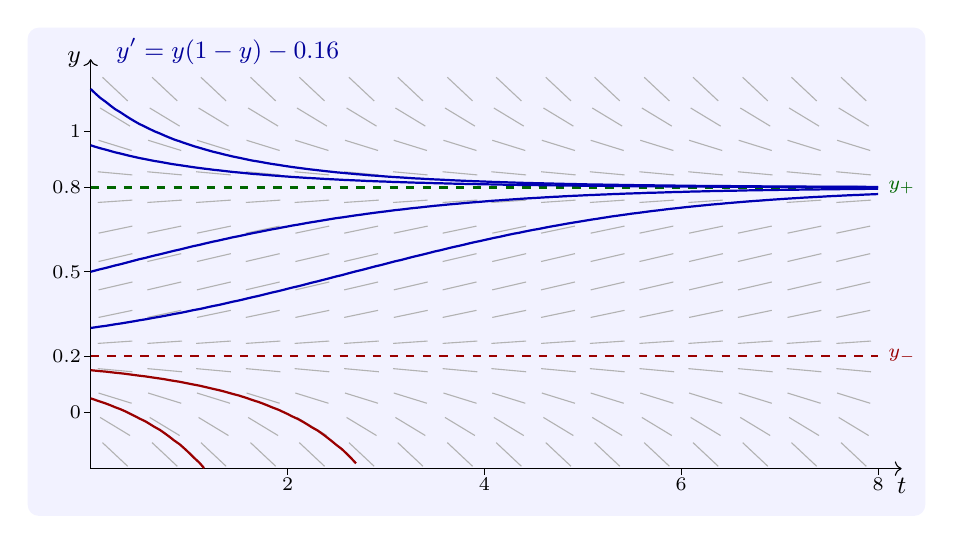
\begin{tikzpicture}
\fill[blue!5,rounded corners=4pt] (-0.8,-0.6) rectangle (10.6,5.6);
\draw[->] (0,0) -- (10.3,0) node[below,font=\small] {$t$};
\draw[->] (0,0) -- (0,5.2) node[left,font=\small] {$y$};
\foreach \v/\y in {0/0.714, 0.2/1.429, 0.5/2.500, 0.8/3.571, 1/4.286}
  \draw (-0.08,\y) -- (0,\y) node[left,font=\scriptsize] {$\v$};
\foreach \v/\x in {2/2.5, 4/5, 6/7.5, 8/10}
  \draw (\x,-0.08) -- (\x,0) node[below,font=\scriptsize] {$\v$};
\draw[gray!60] (0.15,0.33)--(0.47,0.03) (0.12,0.65)--(0.50,0.42) (0.10,0.96)--(0.52,0.83) (0.09,1.27)--(0.53,1.23) (0.09,1.59)--(0.53,1.62) (0.10,1.92)--(0.53,2.01) (0.10,2.27)--(0.53,2.37) (0.10,2.63)--(0.53,2.73) (0.10,2.99)--(0.53,3.08) (0.09,3.38)--(0.53,3.41) (0.09,3.77)--(0.53,3.73) (0.10,4.17)--(0.52,4.04) (0.12,4.58)--(0.50,4.35) (0.15,4.97)--(0.47,4.67) (0.78,0.33)--(1.10,0.03) (0.75,0.65)--(1.13,0.42) (0.73,0.96)--(1.15,0.83) (0.72,1.27)--(1.16,1.23) (0.72,1.59)--(1.16,1.62) (0.72,1.92)--(1.15,2.01) (0.72,2.27)--(1.15,2.37) (0.72,2.63)--(1.15,2.73) (0.72,2.99)--(1.15,3.08) (0.72,3.38)--(1.16,3.41) (0.72,3.77)--(1.16,3.73) (0.73,4.17)--(1.15,4.04) (0.75,4.58)--(1.13,4.35) (0.78,4.97)--(1.10,4.67) (1.40,0.33)--(1.72,0.03) (1.37,0.65)--(1.75,0.42) (1.35,0.96)--(1.77,0.83) (1.34,1.27)--(1.78,1.23) (1.34,1.59)--(1.78,1.62) (1.35,1.92)--(1.78,2.01) (1.35,2.27)--(1.78,2.37) (1.35,2.63)--(1.78,2.73) (1.35,2.99)--(1.78,3.08) (1.34,3.38)--(1.78,3.41) (1.34,3.77)--(1.78,3.73) (1.35,4.17)--(1.77,4.04) (1.37,4.58)--(1.75,4.35) (1.40,4.97)--(1.72,4.67) (2.03,0.33)--(2.35,0.03) (2.00,0.65)--(2.38,0.42) (1.98,0.96)--(2.40,0.83) (1.97,1.27)--(2.41,1.23) (1.97,1.59)--(2.41,1.62) (1.97,1.92)--(2.40,2.01) (1.97,2.27)--(2.40,2.37) (1.97,2.63)--(2.40,2.73) (1.97,2.99)--(2.40,3.08) (1.97,3.38)--(2.41,3.41) (1.97,3.77)--(2.41,3.73) (1.98,4.17)--(2.40,4.04) (2.00,4.58)--(2.38,4.35) (2.03,4.97)--(2.35,4.67) (2.65,0.33)--(2.97,0.03) (2.62,0.65)--(3.00,0.42) (2.60,0.96)--(3.02,0.83) (2.59,1.27)--(3.03,1.23) (2.59,1.59)--(3.03,1.62) (2.60,1.92)--(3.03,2.01) (2.60,2.27)--(3.03,2.37) (2.60,2.63)--(3.03,2.73) (2.60,2.99)--(3.03,3.08) (2.59,3.38)--(3.03,3.41) (2.59,3.77)--(3.03,3.73) (2.60,4.17)--(3.02,4.04) (2.62,4.58)--(3.00,4.35) (2.65,4.97)--(2.97,4.67) (3.28,0.33)--(3.60,0.03) (3.25,0.65)--(3.63,0.42) (3.23,0.96)--(3.65,0.83) (3.22,1.27)--(3.66,1.23) (3.22,1.59)--(3.66,1.62) (3.22,1.92)--(3.65,2.01) (3.22,2.27)--(3.65,2.37) (3.22,2.63)--(3.65,2.73) (3.22,2.99)--(3.65,3.08) (3.22,3.38)--(3.66,3.41) (3.22,3.77)--(3.66,3.73) (3.23,4.17)--(3.65,4.04) (3.25,4.58)--(3.63,4.35) (3.28,4.97)--(3.60,4.67) (3.90,0.33)--(4.22,0.03) (3.87,0.65)--(4.25,0.42) (3.85,0.96)--(4.27,0.83) (3.84,1.27)--(4.28,1.23) (3.84,1.59)--(4.28,1.62) (3.85,1.92)--(4.28,2.01) (3.85,2.27)--(4.28,2.37) (3.85,2.63)--(4.28,2.73) (3.85,2.99)--(4.28,3.08) (3.84,3.38)--(4.28,3.41) (3.84,3.77)--(4.28,3.73) (3.85,4.17)--(4.27,4.04) (3.87,4.58)--(4.25,4.35) (3.90,4.97)--(4.22,4.67) (4.53,0.33)--(4.85,0.03) (4.50,0.65)--(4.88,0.42) (4.48,0.96)--(4.90,0.83) (4.47,1.27)--(4.91,1.23) (4.47,1.59)--(4.91,1.62) (4.47,1.92)--(4.90,2.01) (4.47,2.27)--(4.90,2.37) (4.47,2.63)--(4.90,2.73) (4.47,2.99)--(4.90,3.08) (4.47,3.38)--(4.91,3.41) (4.47,3.77)--(4.91,3.73) (4.48,4.17)--(4.90,4.04) (4.50,4.58)--(4.88,4.35) (4.53,4.97)--(4.85,4.67) (5.15,0.33)--(5.47,0.03) (5.12,0.65)--(5.50,0.42) (5.10,0.96)--(5.52,0.83) (5.09,1.27)--(5.53,1.23) (5.09,1.59)--(5.53,1.62) (5.10,1.92)--(5.53,2.01) (5.10,2.27)--(5.53,2.37) (5.10,2.63)--(5.53,2.73) (5.10,2.99)--(5.53,3.08) (5.09,3.38)--(5.53,3.41) (5.09,3.77)--(5.53,3.73) (5.10,4.17)--(5.52,4.04) (5.12,4.58)--(5.50,4.35) (5.15,4.97)--(5.47,4.67) (5.78,0.33)--(6.10,0.03) (5.75,0.65)--(6.13,0.42) (5.73,0.96)--(6.15,0.83) (5.72,1.27)--(6.16,1.23) (5.72,1.59)--(6.16,1.62) (5.72,1.92)--(6.15,2.01) (5.72,2.27)--(6.15,2.37) (5.72,2.63)--(6.15,2.73) (5.72,2.99)--(6.15,3.08) (5.72,3.38)--(6.16,3.41) (5.72,3.77)--(6.16,3.73) (5.73,4.17)--(6.15,4.04) (5.75,4.58)--(6.13,4.35) (5.78,4.97)--(6.10,4.67) (6.40,0.33)--(6.72,0.03) (6.37,0.65)--(6.75,0.42) (6.35,0.96)--(6.77,0.83) (6.34,1.27)--(6.78,1.23) (6.34,1.59)--(6.78,1.62) (6.35,1.92)--(6.78,2.01) (6.35,2.27)--(6.78,2.37) (6.35,2.63)--(6.78,2.73) (6.35,2.99)--(6.78,3.08) (6.34,3.38)--(6.78,3.41) (6.34,3.77)--(6.78,3.73) (6.35,4.17)--(6.77,4.04) (6.37,4.58)--(6.75,4.35) (6.40,4.97)--(6.72,4.67) (7.03,0.33)--(7.35,0.03) (7.00,0.65)--(7.38,0.42) (6.98,0.96)--(7.40,0.83) (6.97,1.27)--(7.41,1.23) (6.97,1.59)--(7.41,1.62) (6.97,1.92)--(7.40,2.01) (6.97,2.27)--(7.40,2.37) (6.97,2.63)--(7.40,2.73) (6.97,2.99)--(7.40,3.08) (6.97,3.38)--(7.41,3.41) (6.97,3.77)--(7.41,3.73) (6.98,4.17)--(7.40,4.04) (7.00,4.58)--(7.38,4.35) (7.03,4.97)--(7.35,4.67) (7.65,0.33)--(7.97,0.03) (7.62,0.65)--(8.00,0.42) (7.60,0.96)--(8.02,0.83) (7.59,1.27)--(8.03,1.23) (7.59,1.59)--(8.03,1.62) (7.60,1.92)--(8.03,2.01) (7.60,2.27)--(8.03,2.37) (7.60,2.63)--(8.03,2.73) (7.60,2.99)--(8.03,3.08) (7.59,3.38)--(8.03,3.41) (7.59,3.77)--(8.03,3.73) (7.60,4.17)--(8.02,4.04) (7.62,4.58)--(8.00,4.35) (7.65,4.97)--(7.97,4.67) (8.28,0.33)--(8.60,0.03) (8.25,0.65)--(8.63,0.42) (8.23,0.96)--(8.65,0.83) (8.22,1.27)--(8.66,1.23) (8.22,1.59)--(8.66,1.62) (8.22,1.92)--(8.65,2.01) (8.22,2.27)--(8.65,2.37) (8.22,2.63)--(8.65,2.73) (8.22,2.99)--(8.65,3.08) (8.22,3.38)--(8.66,3.41) (8.22,3.77)--(8.66,3.73) (8.23,4.17)--(8.65,4.04) (8.25,4.58)--(8.63,4.35) (8.28,4.97)--(8.60,4.67) (8.90,0.33)--(9.22,0.03) (8.87,0.65)--(9.25,0.42) (8.85,0.96)--(9.27,0.83) (8.84,1.27)--(9.28,1.23) (8.84,1.59)--(9.28,1.62) (8.85,1.92)--(9.28,2.01) (8.85,2.27)--(9.28,2.37) (8.85,2.63)--(9.28,2.73) (8.85,2.99)--(9.28,3.08) (8.84,3.38)--(9.28,3.41) (8.84,3.77)--(9.28,3.73) (8.85,4.17)--(9.27,4.04) (8.87,4.58)--(9.25,4.35) (8.90,4.97)--(9.22,4.67) (9.53,0.33)--(9.85,0.03) (9.50,0.65)--(9.88,0.42) (9.48,0.96)--(9.90,0.83) (9.47,1.27)--(9.91,1.23) (9.47,1.59)--(9.91,1.62) (9.47,1.92)--(9.90,2.01) (9.47,2.27)--(9.90,2.37) (9.47,2.63)--(9.90,2.73) (9.47,2.99)--(9.90,3.08) (9.47,3.38)--(9.91,3.41) (9.47,3.77)--(9.91,3.73) (9.48,4.17)--(9.90,4.04) (9.50,4.58)--(9.88,4.35) (9.53,4.97)--(9.85,4.67);
\draw[red!60!black,dashed,thick] (0,1.429) -- (10,1.429) node[right,font=\scriptsize] {$y_-$};
\draw[green!40!black,dashed,thick] (0,3.571) -- (10,3.571) node[right,font=\scriptsize] {$y_+$};
\draw[red!60!black,thick] plot coordinates {(0.00,0.893) (0.06,0.872) (0.12,0.851) (0.19,0.828) (0.25,0.805) (0.31,0.780) (0.38,0.754) (0.44,0.727) (0.50,0.698) (0.56,0.668) (0.62,0.636) (0.69,0.603) (0.75,0.567) (0.81,0.530) (0.88,0.491) (0.94,0.449) (1.00,0.405) (1.06,0.358) (1.13,0.309) (1.19,0.256) (1.25,0.200) (1.31,0.140) (1.38,0.076) (1.44,0.007)};
\draw[red!60!black,thick] plot coordinates {(0.00,1.250) (0.06,1.244) (0.12,1.238) (0.19,1.232) (0.25,1.225) (0.31,1.218) (0.38,1.211) (0.44,1.204) (0.50,1.196) (0.56,1.188) (0.62,1.180) (0.69,1.172) (0.75,1.163) (0.81,1.154) (0.88,1.144) (0.94,1.135) (1.00,1.124) (1.06,1.114) (1.13,1.103) (1.19,1.091) (1.25,1.079) (1.31,1.067) (1.38,1.054) (1.44,1.040) (1.50,1.026) (1.56,1.012) (1.63,0.996) (1.69,0.981) (1.75,0.964) (1.81,0.947) (1.88,0.929) (1.94,0.910) (2.00,0.890) (2.06,0.869) (2.13,0.847) (2.19,0.825) (2.25,0.801) (2.31,0.776) (2.38,0.750) (2.44,0.722) (2.50,0.694) (2.56,0.663) (2.63,0.631) (2.69,0.598) (2.75,0.562) (2.81,0.524) (2.88,0.485) (2.94,0.443) (3.00,0.398) (3.06,0.351) (3.12,0.301) (3.19,0.248) (3.25,0.191) (3.31,0.131) (3.37,0.066)};
\draw[blue!70!black,thick] plot coordinates {(0.00,1.786) (0.06,1.795) (0.12,1.804) (0.19,1.813) (0.25,1.823) (0.31,1.833) (0.38,1.843) (0.44,1.853) (0.50,1.863) (0.56,1.873) (0.62,1.884) (0.69,1.895) (0.75,1.906) (0.81,1.917) (0.88,1.929) (0.94,1.940) (1.00,1.952) (1.06,1.964) (1.13,1.976) (1.19,1.988) (1.25,2.001) (1.31,2.014) (1.38,2.026) (1.44,2.039) (1.50,2.053) (1.56,2.066) (1.63,2.079) (1.69,2.093) (1.75,2.107) (1.81,2.121) (1.88,2.135) (1.94,2.149) (2.00,2.164) (2.06,2.178) (2.13,2.193) (2.19,2.208) (2.25,2.223) (2.31,2.238) (2.38,2.253) (2.44,2.268) (2.50,2.284) (2.56,2.299) (2.63,2.315) (2.69,2.330) (2.75,2.346) (2.81,2.362) (2.88,2.378) (2.94,2.394) (3.00,2.409) (3.06,2.425) (3.12,2.441) (3.19,2.457) (3.25,2.474) (3.31,2.490) (3.37,2.506) (3.44,2.522) (3.50,2.538) (3.56,2.554) (3.62,2.570) (3.69,2.586) (3.75,2.602) (3.81,2.618) (3.87,2.634) (3.94,2.649) (4.00,2.665) (4.06,2.681) (4.12,2.696) (4.19,2.712) (4.25,2.727) (4.31,2.742) (4.37,2.758) (4.44,2.773) (4.50,2.788) (4.56,2.803) (4.62,2.817) (4.69,2.832) (4.75,2.846) (4.81,2.861) (4.87,2.875) (4.94,2.889) (5.00,2.903) (5.06,2.916) (5.12,2.930) (5.19,2.943) (5.25,2.957) (5.31,2.970) (5.37,2.983) (5.44,2.995) (5.50,3.008) (5.56,3.020) (5.62,3.032) (5.69,3.044) (5.75,3.056) (5.81,3.068) (5.87,3.079) (5.94,3.091) (6.00,3.102) (6.06,3.113) (6.12,3.123) (6.19,3.134) (6.25,3.144) (6.31,3.154) (6.37,3.164) (6.44,3.174) (6.50,3.184) (6.56,3.193) (6.62,3.203) (6.69,3.212) (6.75,3.221) (6.81,3.229) (6.87,3.238) (6.94,3.246) (7.00,3.254) (7.06,3.262) (7.12,3.270) (7.19,3.278) (7.25,3.285) (7.31,3.293) (7.37,3.300) (7.44,3.307) (7.50,3.314) (7.56,3.321) (7.62,3.327) (7.69,3.334) (7.75,3.340) (7.81,3.346) (7.87,3.352) (7.94,3.358) (8.00,3.363) (8.06,3.369) (8.12,3.374) (8.19,3.380) (8.25,3.385) (8.31,3.390) (8.37,3.395) (8.44,3.400) (8.50,3.404) (8.56,3.409) (8.62,3.413) (8.69,3.418) (8.75,3.422) (8.81,3.426) (8.87,3.430) (8.94,3.434) (9.00,3.438) (9.06,3.442) (9.12,3.445) (9.19,3.449) (9.25,3.452) (9.31,3.455) (9.37,3.459) (9.44,3.462) (9.50,3.465) (9.56,3.468) (9.62,3.471) (9.69,3.474) (9.75,3.476) (9.81,3.479) (9.87,3.482) (9.94,3.484) (10.00,3.487) (10.00,3.487)};
\draw[blue!70!black,thick] plot coordinates {(0.00,2.500) (0.06,2.516) (0.12,2.532) (0.19,2.548) (0.25,2.564) (0.31,2.580) (0.38,2.596) (0.44,2.612) (0.50,2.628) (0.56,2.644) (0.62,2.660) (0.69,2.675) (0.75,2.691) (0.81,2.706) (0.88,2.722) (0.94,2.737) (1.00,2.752) (1.06,2.767) (1.13,2.782) (1.19,2.797) (1.25,2.812) (1.31,2.827) (1.38,2.841) (1.44,2.856) (1.50,2.870) (1.56,2.884) (1.63,2.898) (1.69,2.912) (1.75,2.925) (1.81,2.939) (1.88,2.952) (1.94,2.965) (2.00,2.978) (2.06,2.991) (2.13,3.004) (2.19,3.016) (2.25,3.028) (2.31,3.040) (2.38,3.052) (2.44,3.064) (2.50,3.075) (2.56,3.087) (2.63,3.098) (2.69,3.109) (2.75,3.120) (2.81,3.130) (2.88,3.141) (2.94,3.151) (3.00,3.161) (3.06,3.171) (3.12,3.181) (3.19,3.190) (3.25,3.199) (3.31,3.208) (3.37,3.217) (3.44,3.226) (3.50,3.235) (3.56,3.243) (3.62,3.251) (3.69,3.260) (3.75,3.267) (3.81,3.275) (3.87,3.283) (3.94,3.290) (4.00,3.297) (4.06,3.305) (4.12,3.311) (4.19,3.318) (4.25,3.325) (4.31,3.331) (4.37,3.338) (4.44,3.344) (4.50,3.350) (4.56,3.356) (4.62,3.361) (4.69,3.367) (4.75,3.373) (4.81,3.378) (4.87,3.383) (4.94,3.388) (5.00,3.393) (5.06,3.398) (5.12,3.403) (5.19,3.407) (5.25,3.412) (5.31,3.416) (5.37,3.420) (5.44,3.425) (5.50,3.429) (5.56,3.433) (5.62,3.436) (5.69,3.440) (5.75,3.444) (5.81,3.447) (5.87,3.451) (5.94,3.454) (6.00,3.458) (6.06,3.461) (6.12,3.464) (6.19,3.467) (6.25,3.470) (6.31,3.473) (6.37,3.475) (6.44,3.478) (6.50,3.481) (6.56,3.483) (6.62,3.486) (6.69,3.488) (6.75,3.491) (6.81,3.493) (6.87,3.495) (6.94,3.497) (7.00,3.499) (7.06,3.502) (7.12,3.504) (7.19,3.505) (7.25,3.507) (7.31,3.509) (7.37,3.511) (7.44,3.513) (7.50,3.514) (7.56,3.516) (7.62,3.518) (7.69,3.519) (7.75,3.521) (7.81,3.522) (7.87,3.524) (7.94,3.525) (8.00,3.526) (8.06,3.528) (8.12,3.529) (8.19,3.530) (8.25,3.531) (8.31,3.533) (8.37,3.534) (8.44,3.535) (8.50,3.536) (8.56,3.537) (8.62,3.538) (8.69,3.539) (8.75,3.540) (8.81,3.541) (8.87,3.542) (8.94,3.542) (9.00,3.543) (9.06,3.544) (9.12,3.545) (9.19,3.546) (9.25,3.546) (9.31,3.547) (9.37,3.548) (9.44,3.549) (9.50,3.549) (9.56,3.550) (9.62,3.551) (9.69,3.551) (9.75,3.552) (9.81,3.552) (9.87,3.553) (9.94,3.553) (10.00,3.554) (10.00,3.554)};
\draw[blue!70!black,thick] plot coordinates {(0.00,4.107) (0.06,4.087) (0.12,4.069) (0.19,4.051) (0.25,4.034) (0.31,4.017) (0.38,4.001) (0.44,3.986) (0.50,3.971) (0.56,3.958) (0.62,3.944) (0.69,3.931) (0.75,3.919) (0.81,3.907) (0.88,3.896) (0.94,3.885) (1.00,3.874) (1.06,3.864) (1.13,3.854) (1.19,3.845) (1.25,3.836) (1.31,3.827) (1.38,3.818) (1.44,3.810) (1.50,3.803) (1.56,3.795) (1.63,3.788) (1.69,3.781) (1.75,3.774) (1.81,3.767) (1.88,3.761) (1.94,3.755) (2.00,3.749) (2.06,3.743) (2.13,3.738) (2.19,3.733) (2.25,3.728) (2.31,3.723) (2.38,3.718) (2.44,3.713) (2.50,3.709) (2.56,3.704) (2.63,3.700) (2.69,3.696) (2.75,3.692) (2.81,3.689) (2.88,3.685) (2.94,3.681) (3.00,3.678) (3.06,3.675) (3.12,3.672) (3.19,3.668) (3.25,3.665) (3.31,3.663) (3.37,3.660) (3.44,3.657) (3.50,3.654) (3.56,3.652) (3.62,3.649) (3.69,3.647) (3.75,3.645) (3.81,3.642) (3.87,3.640) (3.94,3.638) (4.00,3.636) (4.06,3.634) (4.12,3.632) (4.19,3.630) (4.25,3.629) (4.31,3.627) (4.37,3.625) (4.44,3.624) (4.50,3.622) (4.56,3.620) (4.62,3.619) (4.69,3.618) (4.75,3.616) (4.81,3.615) (4.87,3.614) (4.94,3.612) (5.00,3.611) (5.06,3.610) (5.12,3.609) (5.19,3.608) (5.25,3.606) (5.31,3.605) (5.37,3.604) (5.44,3.603) (5.50,3.602) (5.56,3.602) (5.62,3.601) (5.69,3.600) (5.75,3.599) (5.81,3.598) (5.87,3.597) (5.94,3.597) (6.00,3.596) (6.06,3.595) (6.12,3.594) (6.19,3.594) (6.25,3.593) (6.31,3.592) (6.37,3.592) (6.44,3.591) (6.50,3.591) (6.56,3.590) (6.62,3.589) (6.69,3.589) (6.75,3.588) (6.81,3.588) (6.87,3.587) (6.94,3.587) (7.00,3.586) (7.06,3.586) (7.12,3.586) (7.19,3.585) (7.25,3.585) (7.31,3.584) (7.37,3.584) (7.44,3.584) (7.50,3.583) (7.56,3.583) (7.62,3.583) (7.69,3.582) (7.75,3.582) (7.81,3.582) (7.87,3.581) (7.94,3.581) (8.00,3.581) (8.06,3.580) (8.12,3.580) (8.19,3.580) (8.25,3.580) (8.31,3.579) (8.37,3.579) (8.44,3.579) (8.50,3.579) (8.56,3.578) (8.62,3.578) (8.69,3.578) (8.75,3.578) (8.81,3.578) (8.87,3.577) (8.94,3.577) (9.00,3.577) (9.06,3.577) (9.12,3.577) (9.19,3.577) (9.25,3.576) (9.31,3.576) (9.37,3.576) (9.44,3.576) (9.50,3.576) (9.56,3.576) (9.62,3.576) (9.69,3.576) (9.75,3.575) (9.81,3.575) (9.87,3.575) (9.94,3.575) (10.00,3.575) (10.00,3.575)};
\draw[blue!70!black,thick] plot coordinates {(0.00,4.821) (0.06,4.764) (0.12,4.710) (0.19,4.659) (0.25,4.611) (0.31,4.566) (0.38,4.524) (0.44,4.484) (0.50,4.446) (0.56,4.410) (0.62,4.376) (0.69,4.343) (0.75,4.313) (0.81,4.284) (0.88,4.256) (0.94,4.229) (1.00,4.204) (1.06,4.180) (1.13,4.157) (1.19,4.135) (1.25,4.115) (1.31,4.095) (1.38,4.075) (1.44,4.057) (1.50,4.040) (1.56,4.023) (1.63,4.007) (1.69,3.991) (1.75,3.977) (1.81,3.963) (1.88,3.949) (1.94,3.936) (2.00,3.923) (2.06,3.911) (2.13,3.900) (2.19,3.889) (2.25,3.878) (2.31,3.868) (2.38,3.858) (2.44,3.848) (2.50,3.839) (2.56,3.830) (2.63,3.821) (2.69,3.813) (2.75,3.805) (2.81,3.798) (2.88,3.790) (2.94,3.783) (3.00,3.776) (3.06,3.770) (3.12,3.763) (3.19,3.757) (3.25,3.751) (3.31,3.746) (3.37,3.740) (3.44,3.735) (3.50,3.729) (3.56,3.724) (3.62,3.720) (3.69,3.715) (3.75,3.710) (3.81,3.706) (3.87,3.702) (3.94,3.698) (4.00,3.694) (4.06,3.690) (4.12,3.686) (4.19,3.683) (4.25,3.679) (4.31,3.676) (4.37,3.673) (4.44,3.670) (4.50,3.667) (4.56,3.664) (4.62,3.661) (4.69,3.658) (4.75,3.655) (4.81,3.653) (4.87,3.650) (4.94,3.648) (5.00,3.646) (5.06,3.643) (5.12,3.641) (5.19,3.639) (5.25,3.637) (5.31,3.635) (5.37,3.633) (5.44,3.631) (5.50,3.629) (5.56,3.628) (5.62,3.626) (5.69,3.624) (5.75,3.623) (5.81,3.621) (5.87,3.620) (5.94,3.618) (6.00,3.617) (6.06,3.615) (6.12,3.614) (6.19,3.613) (6.25,3.611) (6.31,3.610) (6.37,3.609) (6.44,3.608) (6.50,3.607) (6.56,3.606) (6.62,3.605) (6.69,3.604) (6.75,3.603) (6.81,3.602) (6.87,3.601) (6.94,3.600) (7.00,3.599) (7.06,3.598) (7.12,3.598) (7.19,3.597) (7.25,3.596) (7.31,3.595) (7.37,3.595) (7.44,3.594) (7.50,3.593) (7.56,3.593) (7.62,3.592) (7.69,3.591) (7.75,3.591) (7.81,3.590) (7.87,3.590) (7.94,3.589) (8.00,3.589) (8.06,3.588) (8.12,3.588) (8.19,3.587) (8.25,3.587) (8.31,3.586) (8.37,3.586) (8.44,3.585) (8.50,3.585) (8.56,3.584) (8.62,3.584) (8.69,3.584) (8.75,3.583) (8.81,3.583) (8.87,3.583) (8.94,3.582) (9.00,3.582) (9.06,3.582) (9.12,3.581) (9.19,3.581) (9.25,3.581) (9.31,3.581) (9.37,3.580) (9.44,3.580) (9.50,3.580) (9.56,3.579) (9.62,3.579) (9.69,3.579) (9.75,3.579) (9.81,3.579) (9.87,3.578) (9.94,3.578) (10.00,3.578) (10.00,3.578)};
\node[font=\small\bfseries,anchor=west,blue!60!black] at (0.2,5.3) {$y' = y(1 - y) - 0.16$};
\end{tikzpicture}
\caption{Direction field and solutions of the harvesting equation with $h = 0.16$, for which $y_- = 0.2$ and $y_+ = 0.8$. Each short segment has the slope $f(y)$ that a
solution through that point must have. Solutions starting above $0.2$ approach $0.8$; those starting below $0.2$ fall towards collapse.}
\label{fig:dirfield}
\end{figure}

\begin{figure}[H]
\centering
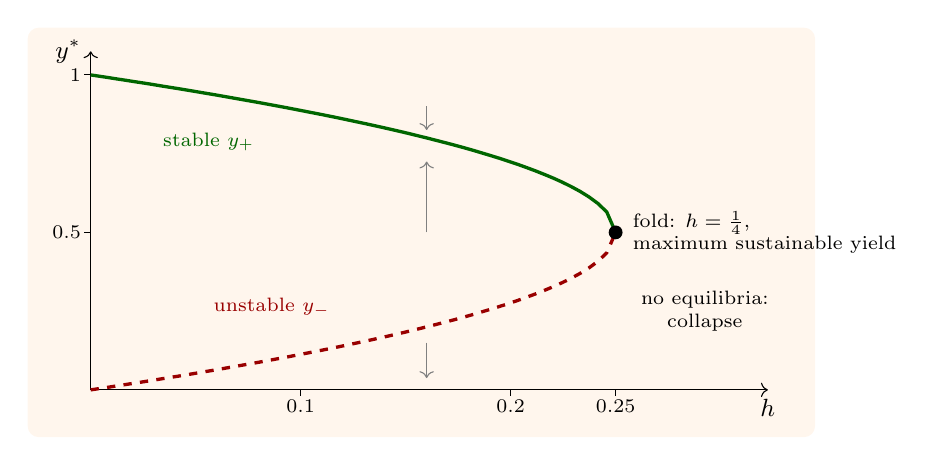
\begin{tikzpicture}
\fill[orange!7,rounded corners=4pt] (-0.8,-0.6) rectangle (9.2,4.6);
\draw[->] (0,0) -- (8.6,0) node[below,font=\small] {$h$};
\draw[->] (0,0) -- (0,4.3) node[left,font=\small] {$y^*$};
\foreach \v/\x in {0.1/2.667, 0.2/5.333, 0.25/6.667}
  \draw (\x,-0.08) -- (\x,0) node[below,font=\scriptsize] {$\v$};
\foreach \v/\y in {0.5/2, 1/4}
  \draw (-0.08,\y) -- (0,\y) node[left,font=\scriptsize] {$\v$};
\draw[green!40!black,very thick] plot coordinates {(0.000,4.000) (0.113,3.983) (0.226,3.966) (0.339,3.948) (0.452,3.931) (0.565,3.913) (0.678,3.896) (0.791,3.878) (0.904,3.859) (1.017,3.841) (1.130,3.823) (1.243,3.804) (1.356,3.785) (1.469,3.766) (1.582,3.747) (1.695,3.727) (1.808,3.707) (1.921,3.687) (2.034,3.667) (2.147,3.647) (2.260,3.626) (2.373,3.605) (2.486,3.584) (2.599,3.562) (2.712,3.540) (2.825,3.518) (2.938,3.496) (3.051,3.473) (3.164,3.450) (3.277,3.426) (3.390,3.402) (3.503,3.378) (3.616,3.353) (3.729,3.328) (3.842,3.302) (3.955,3.276) (4.068,3.249) (4.181,3.221) (4.294,3.193) (4.407,3.164) (4.520,3.135) (4.633,3.105) (4.746,3.074) (4.859,3.042) (4.972,3.008) (5.085,2.974) (5.198,2.939) (5.311,2.902) (5.424,2.864) (5.537,2.823) (5.650,2.781) (5.763,2.736) (5.876,2.689) (5.989,2.638) (6.102,2.582) (6.215,2.521) (6.328,2.451) (6.441,2.368) (6.554,2.260) (6.667,2.000)};
\draw[red!60!black,very thick,dashed] plot coordinates {(0.000,0.000) (0.113,0.017) (0.226,0.034) (0.339,0.052) (0.452,0.069) (0.565,0.087) (0.678,0.104) (0.791,0.122) (0.904,0.141) (1.017,0.159) (1.130,0.177) (1.243,0.196) (1.356,0.215) (1.469,0.234) (1.582,0.253) (1.695,0.273) (1.808,0.293) (1.921,0.313) (2.034,0.333) (2.147,0.353) (2.260,0.374) (2.373,0.395) (2.486,0.416) (2.599,0.438) (2.712,0.460) (2.825,0.482) (2.938,0.504) (3.051,0.527) (3.164,0.550) (3.277,0.574) (3.390,0.598) (3.503,0.622) (3.616,0.647) (3.729,0.672) (3.842,0.698) (3.955,0.724) (4.068,0.751) (4.181,0.779) (4.294,0.807) (4.407,0.836) (4.520,0.865) (4.633,0.895) (4.746,0.926) (4.859,0.958) (4.972,0.992) (5.085,1.026) (5.198,1.061) (5.311,1.098) (5.424,1.136) (5.537,1.177) (5.650,1.219) (5.763,1.264) (5.876,1.311) (5.989,1.362) (6.102,1.418) (6.215,1.479) (6.328,1.549) (6.441,1.632) (6.554,1.740) (6.667,2.000)};
\fill (6.667,2) circle (2.5pt) node[right,font=\scriptsize,align=left] {\ fold: $h = \frac14$,\\ \ maximum sustainable yield};
\draw[->,gray] (4.267,3.6) -- (4.267,3.3); \draw[->,gray] (4.267,2.0) -- (4.267,2.9);
\draw[->,gray] (4.267,0.6) -- (4.267,0.15);
\node[font=\scriptsize,green!40!black] at (1.5,3.15) {stable $y_+$};
\node[font=\scriptsize,red!60!black] at (2.3,1.05) {unstable $y_-$};
\node[font=\scriptsize,align=center] at (7.8,1.0) {no equilibria:\\ collapse};
\end{tikzpicture}
\caption{The saddle-node bifurcation in the harvesting model. For each harvest rate $h$ the equilibria are the points above it; the arrows show the direction of
motion on the phase line at $h = 0.16$. At $h = \frac14$ the stable and unstable equilibria collide and vanish.}
\label{fig:bifharvest}
\end{figure}

\subsection{First-order equations in software}
\label{ssec:software1}

The panels use Python with the libraries SymPy (symbolic mathematics), NumPy and SciPy (numerical computation). Each shows the commands as typed at the
Python prompt and the output they print, and ends with the equivalent MATLAB or Octave commands.

\begin{software}[Symbolic solution with SymPy]
\label{sw:sympy1}
\texttt{dsolve} recognises the standard types; \texttt{checkodesol} substitutes the answer back into the equation. For the exact equation of Example~\ref{ex:exact} the
potential is built by the two integrations in the proof of Theorem~\ref{thm:exact}:
{\small\begin{verbatim}
>>> import sympy as sp
>>> t = sp.symbols('t'); y = sp.Function('y')
>>> lin = sp.dsolve(y(t).diff(t) + 2*y(t) - sp.exp(-t), y(t)); lin
Eq(y(t), (C1*exp(-t) + 1)*exp(-t))
>>> sp.checkodesol(y(t).diff(t) + 2*y(t) - sp.exp(-t), lin)
(True, 0)
>>> ber = sp.dsolve(y(t).diff(t) - y(t) + y(t)**3, y(t)); ber[1]   # y > 0
Eq(y(t), sqrt(-exp(2*t)/(C1 - exp(2*t))))
>>> x, v = sp.symbols('x v')               # exact: M dx + N dv = 0
>>> M, N = 2*x*v, x**2 + 3*v**2
>>> sp.diff(M, v) == sp.diff(N, x)          # the exactness test
True
>>> F = sp.integrate(M, x)                  # M in x, then the v part
>>> F = F + sp.integrate(sp.simplify(N - sp.diff(F, v)), v); F
v**3 + v*x**2
\end{verbatim}}
\textbf{Reading the output.} The linear equation $y' + 2y = e^{-t}$ has general solution $y = e^{-t} + C_1e^{-2t}$, printed in the factored form $(C_1e^{-t} + 1)e^{-t}$, and \texttt{checkodesol}
confirms it with residual $0$. For the Bernoulli equation $y' = y - y^3$, the positive branch is $y = \bigl(e^{2t}/(e^{2t} - C_1)\bigr)^{1/2}$, which the substitution $w = y^{-2}$ of
Theorem~\ref{thm:bernoulli} produces by hand; every positive solution tends to $1$. The potential of the exact equation is $x^2y + y^3$, as in Example~\ref{ex:exact} (with $v$ for $y$). Asking \texttt{dsolve}
for the exact equation itself returns the three roots of the cubic $y^3 + x^2y - C = 0$ in Cardano's form, a reminder that the implicit form $F(x, y) = C$ is often the
better answer.

\textbf{MATLAB/Octave:} \texttt{syms y(t); dsolve(diff(y) + 2*y == exp(-t))} with the Symbolic Math Toolbox (or the \texttt{symbolic} package in Octave).
\end{software}

\begin{software}[Numerical solution with \texttt{solve\_ivp}]
\label{sw:solveivp1}
The logistic equation with $r = 1$, $K = 100$, $y_0 = 10$, solved numerically and compared with the exact solution of Example~\ref{ex:logistic}:
{\small\begin{verbatim}
>>> import numpy as np
>>> from scipy.integrate import solve_ivp
>>> r, K, y0 = 1.0, 100.0, 10.0
>>> exact = lambda t: K / (1 + (K / y0 - 1) * np.exp(-r * t))
>>> sol = solve_ivp(lambda t, y: r * y * (1 - y / K), (0, 10), [y0],
...                 rtol=1e-8, atol=1e-10, dense_output=True)
>>> ts = np.array([0, 2, 4, 6, 10])
>>> np.round(np.c_[ts, sol.sol(ts)[0], exact(ts)], 4)
array([[ 0.    , 10.    , 10.    ],
       [ 2.    , 45.0853, 45.0853],
       [ 4.    , 85.8486, 85.8486],
       [ 6.    , 97.8178, 97.8178],
       [10.    , 99.9592, 99.9592]])
>>> sol.nfev, np.max(np.abs(sol.sol(ts)[0] - exact(ts)))
(314, 8.665153856668439e-07)
\end{verbatim}}
\textbf{Reading the output.} The numerical and exact values agree to four decimals: the largest difference at the five times is $8.7 \times 10^{-7}$, within the requested
tolerances. The solver, an adaptive Runge--Kutta method of order $5(4)$ that is described in the last section, used $314$ evaluations of $f$. The population passes
$K/2 = 50$ just after $t = 2$, at $t^* = \log 9 = 2.20$, and reaches $99.96$ by $t = 10$. \texttt{dense\_output=True} returns an interpolant, \texttt{sol.sol}, so the solution can be
evaluated at any time, not just at the solver's own steps.

\textbf{MATLAB/Octave:} \texttt{opts = odeset('RelTol', 1e-8);} then \texttt{[t, y] = ode45(@(t, y) y.*(1 - y/100), [0 10], 10, opts)}.
\end{software}

\begin{software}[Equilibria and the harvesting bifurcation]
\label{sw:harvest}
The equilibria of $y' = y(1 - y) - h$ and the signs of $f'$ at them, for three harvest rates:
{\small\begin{verbatim}
>>> u, h = sp.symbols('u h', real=True)
>>> f = u * (1 - u) - h
>>> eq = sp.solve(f, u); eq
[1/2 - sqrt(1 - 4*h)/2, sqrt(1 - 4*h)/2 + 1/2]
>>> for hv in [0.16, 0.25, 0.3]:
...     roots = [complex(e.subs(h, hv)) for e in eq]
...     slopes = [complex(sp.diff(f, u).subs({u: rt, h: hv})) for rt in roots]
...     real = [abs(rt.imag) < 1e-12 for rt in roots]
...     print(hv, [round(rt.real, 3) for rt, ok in zip(roots, real) if ok],
...           [round(s.real, 3) for s, ok in zip(slopes, real) if ok])
...
0.16 [0.2, 0.8] [0.6, -0.6]
0.25 [0.5, 0.5] [0.0, 0.0]
0.3 [] []
\end{verbatim}}
\textbf{Reading the output.} For $h = 0.16$ the equilibria are $0.2$ and $0.8$, with $f' = 0.6$ (unstable) and $-0.6$ (stable), as in Figure~\ref{fig:dirfield}. At $h = 0.25$ they coincide at $0.5$,
where $f' = 0$ and the linear test of Theorem~\ref{thm:phaseline}(iv) fails. For $h = 0.3$ the roots are complex and there are no equilibria at all: the population
declines to zero from any starting value.

\textbf{MATLAB/Octave:} \texttt{roots([-1 1 -0.16])} for the equilibria at $h = 0.16$.
\end{software}

\subsection{Practice Problems}

\begin{problem}
Solve $y' + y\tan t = \sec t$, $y(0) = 2$, on $(-\pi/2, \pi/2)$, and explain why the solution cannot be continued past $\pm\pi/2$ by the theorem.
\end{problem}

\begin{solution}
Here $p = \tan t$, $P(t) = \int_0^t\tan s\,ds = -\log\cos t$, and $e^{P} = \sec t$. By Theorem~\ref{thm:linear1}, $y = \cos t\,\bigl(2 + \int_0^t\sec^2s\,ds\bigr) = \cos t(2 + \tan t) = 2\cos t + \sin t$. The theorem
guarantees the solution on the largest interval containing $0$ on which $\tan t$ and $\sec t$ are continuous, which is $(-\pi/2, \pi/2)$. The formula $2\cos t + \sin t$ happens to extend
smoothly beyond, but the equation itself is undefined at $\pm\pi/2$, so the theorem says nothing there.
\end{solution}

\begin{problem}
\label{prob:blowup}
Solve $y' = t y^2$, $y(0) = y_0$, and find the interval of existence. Compare $y_0 = 1$ and $y_0 = -1$.
\end{problem}

\begin{solution}
For $y_0 \neq 0$, separation gives $-1/y = t^2/2 - 1/y_0$, so $y = 2y_0/(2 - y_0t^2)$; for $y_0 = 0$, $y \equiv 0$. With $y_0 = 1$, $y = 2/(2 - t^2)$, which exists only on $(-\sqrt2, \sqrt2)$ and tends to $+\infty$
at the ends: the solution \textbf{blows up} in finite time although $f(t, y) = ty^2$ is smooth everywhere. With $y_0 = -1$, $y = -2/(2 + t^2)$, which exists for all $t$ and tends to $0$. The
interval of existence of a non-linear equation depends on the initial value, unlike the linear case.
\end{solution}

\begin{problem}
Show that $(3x^2 + y\cos x)\,dx + (\sin x - 4y^3)\,dy = 0$ is exact and find its solutions.
\end{problem}

\begin{solution}
$M_y = \cos x = N_x$. Integrating $M$ in $x$: $F = x^3 + y\sin x + \psi(y)$, and $F_y = \sin x + \psi' = \sin x - 4y^3$ gives $\psi = -y^4$. The solutions satisfy $x^3 + y\sin x - y^4 = C$.
\end{solution}

\begin{problem}
Find an integrating factor for $(x^2 + y^2 + x)\,dx + xy\,dy = 0$ and solve the equation.
\end{problem}

\begin{solution}
$M_y = 2y$, $N_x = y$, and $(M_y - N_x)/N = y/(xy) = 1/x$, a function of $x$ alone, so $\mu = x$ by Theorem~\ref{thm:intfactor}. Then $(x^3 + xy^2 + x^2)\,dx + x^2y\,dy = 0$ is exact, with
$F = \frac14x^4 + \frac12x^2y^2 + \frac13x^3$, and the solutions satisfy $3x^4 + 6x^2y^2 + 4x^3 = C$.
\end{solution}

\begin{problem}
The Riccati equation $y' = 1 + t^2 - y^2$ has the solution $y_1 = t$. Find the general solution.
\end{problem}

\begin{solution}
Here $q_0 = 1 + t^2$, $q_1 = 0$, $q_2 = -1$. By Theorem~\ref{thm:riccati}(i), $y = t + 1/v$ with $v' = -(0 + 2(-1)t)v - (-1) = 2tv + 1$. The integrating factor is $e^{-t^2}$, so
$v = e^{t^2}\bigl(C + \int_0^te^{-s^2}\,ds\bigr)$ and
\[
y = t + \frac{e^{-t^2}}{C + \int_0^te^{-s^2}\,ds} .
\]
The integral is $\frac{\sqrt\pi}{2}\operatorname{erf}(t)$, a non-elementary function, as Theorem~\ref{thm:riccati}(ii) leads one to expect.
\end{solution}

\begin{problem}
For $y' = y^2(1 - y)$, draw the phase line, classify the equilibria, and describe the solutions with $y(0) = -0.1$, $0.1$ and $1.5$.
\end{problem}

\begin{solution}
The equilibria are $0$ and $1$. The sign of $f$ is positive for $y < 0$ and for $0 < y < 1$, and negative for $y > 1$. So $1$ is asymptotically stable ($f'(1) = -1$), and $0$ is
semi-stable ($f'(0) = 0$): solutions approach it from below and leave it above. Starting at $-0.1$, the solution increases towards $0$; at $0.1$ it increases towards $1$; at
$1.5$ it decreases towards $1$. The first two show that a solution starting near $0$ on one side tends to $0$ and on the other side goes away from it.
\end{solution}

\begin{problem}
\label{prob:harvestprop}
Modify Example~\ref{ex:harvest} so that the harvest is proportional to the stock, $y' = y(1 - y) - Ey$, with effort $E \geq 0$. Find the equilibria and their stability,
the sustainable yield $Ey^*$ at the stable equilibrium, and the effort that maximises it. Why is proportional harvesting safer than a fixed quota?
\end{problem}

\begin{solution}
The equilibria are $0$ and $y^* = 1 - E$ (for $E < 1$). With $f'(y) = 1 - E - 2y$, $f'(0) = 1 - E > 0$ and $f'(1 - E) = -(1 - E) < 0$, so $y^*$ is stable and $0$ unstable. The yield is
$E(1 - E)$, maximised at $E = \frac12$ with yield $\frac14$, the same maximum as before. But now, for every $E < 1$, any positive stock recovers to $y^* > 0$: there is no cliff,
because the catch falls automatically when the stock falls. Here the equilibria $0$ and $1 - E$ exchange stability at $E = 1$ instead of disappearing (a transcritical
bifurcation), and a fixed quota $h$ near $\frac14$ is dangerous because a small error or shock pushes the stock below the unstable $y_-$.
\end{solution}

%======================================================================
\section{Existence and Uniqueness}
\label{sec:exist}

Example~\ref{ex:nonunique} showed that an initial value problem with a perfectly continuous right-hand side can have infinitely many solutions, and
Problem~\ref{prob:blowup} that a solution of a smooth equation can cease to exist after a finite time. Before solutions can be studied, it must be known when they
exist, when they are unique, and how they depend on the data. This section answers these questions for the general system
\[
x' = f(t, x), \qquad x(t_0) = x_0, \qquad x \in \mathbb R^n .
\]
The answers are the foundation of everything that follows: they justify the numerical methods, the phase-plane pictures and the stability theory,
all of which assume that a state determines its future.

Throughout, $\|\cdot\|$ is a norm on $\mathbb R^n$ (any norm will do, since all are equivalent), and for a continuous function $\phi$ on an interval $J$, $\|\phi\|_\infty = \sup_{t \in J}\|\phi(t)\|$.

\subsection{The integral equation}
\label{ssec:integral}

\begin{lem}
\label{lem:integral}
Let $f$ be continuous on an open set $D \subseteq \mathbb R \times \mathbb R^n$ containing $(t_0, x_0)$, and let $J$ be an interval containing $t_0$. A continuous function $\phi\colon J \to \mathbb R^n$
with graph in $D$ solves the initial value problem on $J$ if and only if
\[
\phi(t) = x_0 + \int_{t_0}^tf\bigl(s, \phi(s)\bigr)\,ds \qquad\text{for all } t \in J .
\]
\end{lem}

\begin{proof}
If $\phi$ solves the problem, then $\phi'(s) = f(s, \phi(s))$ is continuous, and integrating from $t_0$ to $t$ gives the equation, by the fundamental theorem of calculus. Conversely,
if $\phi$ is continuous and satisfies the equation, the integrand $s \mapsto f(s, \phi(s))$ is continuous, so the right-hand side is differentiable with derivative $f(t, \phi(t))$, and
$\phi(t_0) = x_0$.
\end{proof}

The lemma converts a differential equation into a fixed-point problem: $\phi$ is a solution if and only if $\phi = T\phi$, where
\[
(T\phi)(t) = x_0 + \int_{t_0}^tf\bigl(s, \phi(s)\bigr)\,ds .
\]
The integral equation needs only continuity of $\phi$, not differentiability, which is what makes it the natural setting for limits.

\subsection{Lipschitz conditions}
\label{ssec:lipschitz}

\begin{defn}
$f$ is \textbf{Lipschitz in $x$} on a set $R$ with constant $L$ if
\[
\|f(t, x) - f(t, y)\| \leq L\|x - y\| \qquad\text{for all } (t, x), (t, y) \in R ,
\]
and \textbf{locally Lipschitz} on $D$ if every point of $D$ has a neighbourhood on which $f$ is Lipschitz in $x$.
\end{defn}

\begin{lem}
\label{lem:c1lip}
If $f$ and its partial derivatives $\partial f_i/\partial x_j$ are continuous on $D$, then $f$ is locally Lipschitz. On a set $R = [t_0 - a, t_0 + a] \times \bar B(x_0, b)$ contained in $D$, one may
take $L = \max_R\|D_xf(t, x)\|$, the largest operator norm of the Jacobian matrix.
\end{lem}

\begin{proof}
The ball $\bar B(x_0, b)$ is convex, so for $x, y$ in it the segment $x + \theta(y - x)$, $0 \leq \theta \leq 1$, stays in $R$. By the fundamental theorem of calculus applied to $\theta \mapsto f(t, x + \theta(y - x))$,
\[
f(t, y) - f(t, x) = \int_0^1D_xf\bigl(t, x + \theta(y - x)\bigr)(y - x)\,d\theta ,
\]
whose norm is at most $\max_R\|D_xf\|\,\|y - x\|$. The maximum exists because $D_xf$ is continuous on the compact set $R$. Every point of $D$ has such a compact neighbourhood.
\end{proof}

\begin{exa}
\label{ex:lipschitz}
\begin{enumerate}[label=(\alph*)]
\item $f(x) = 1 + x^2$ is Lipschitz on $|x| \leq b$ with $L = 2b$, since $|x^2 - y^2| = |x + y||x - y|$; it is locally but not globally Lipschitz on $\mathbb R$.
\item $f(x) = \sin x$ is globally Lipschitz with $L = 1$, and a linear $f(t, x) = A(t)x$ is Lipschitz on $[\alpha, \beta] \times \mathbb R^n$ with $L = \max\|A(t)\|$.
\item $f(x) = 3x^{2/3}$ is not Lipschitz near $0$: $|f(x) - f(0)|/|x - 0| = 3|x|^{-1/3} \to \infty$. Nor is $\sqrt{|x|}$. Both are continuous, and both have non-unique solutions from $0$.
\end{enumerate}
\end{exa}

\subsection{The Picard--Lindel\"of theorem}
\label{ssec:picard}

Fix the rectangle (in $\mathbb R^{n+1}$, a cylinder)
\[
R = \bigl\{(t, x) : |t - t_0| \leq a,\ \|x - x_0\| \leq b\bigr\}, \qquad M = \max_R\|f\|, \qquad \alpha = \min\Bigl(a, \frac bM\Bigr).
\]
A solution starting at $x_0$ moves with speed at most $M$, so in time $|t - t_0| \leq b/M$ it cannot leave the ball of radius $b$; this is why the interval of existence is
$\alpha$ rather than $a$ (Figure~\ref{fig:cone}).

\begin{figure}[H]
\centering
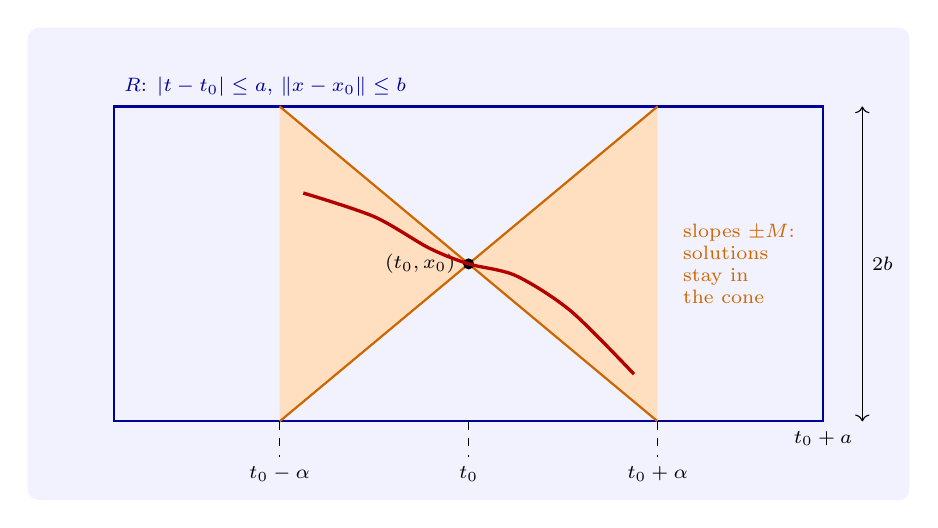
\begin{tikzpicture}[x=1cm,y=1cm]
\fill[blue!5,rounded corners=4pt] (-0.6,-0.7) rectangle (10.6,5.3);
\draw[thick,blue!60!black] (0.5,0.3) rectangle (9.5,4.3);
\node[font=\scriptsize,blue!60!black,anchor=south west] at (0.5,4.3) {$R$: $|t - t_0| \leq a$, $\|x - x_0\| \leq b$};
\fill[orange!25] (5,2.3) -- (7.4,4.3) -- (7.4,0.3) -- cycle;
\fill[orange!25] (5,2.3) -- (2.6,4.3) -- (2.6,0.3) -- cycle;
\draw[orange!80!black,thick] (2.6,4.3) -- (7.4,0.3) (2.6,0.3) -- (7.4,4.3);
\draw[dashed] (2.6,0.3) -- (2.6,-0.15) (7.4,0.3) -- (7.4,-0.15) (5,0.3) -- (5,-0.15);
\node[font=\scriptsize,below] at (5,-0.15) {$t_0$};
\node[font=\scriptsize,below] at (7.4,-0.15) {$t_0 + \alpha$};
\node[font=\scriptsize,below] at (2.6,-0.15) {$t_0 - \alpha$};
\node[font=\scriptsize,below] at (9.5,0.3) {$t_0 + a$};
\fill (5,2.3) circle (2pt) node[left,font=\scriptsize] {$(t_0, x_0)$\,};
\draw[red!70!black,very thick] plot[smooth] coordinates {(2.9,3.2) (3.8,2.9) (4.5,2.5) (5,2.3) (5.6,2.15) (6.3,1.7) (7.1,0.9)};
\node[font=\scriptsize,orange!80!black,align=left,anchor=west] at (7.6,2.3) {slopes $\pm M$:\\ solutions\\ stay in\\ the cone};
\draw[<->] (10.0,0.3) -- node[right,font=\scriptsize] {$2b$} (10.0,4.3);
\end{tikzpicture}
\caption{The interval of existence in the Picard--Lindel\"of theorem. A solution through $(t_0, x_0)$ has $\|x'\| \leq M$ while it stays in $R$, so its graph lies in the double cone
of slopes $\pm M$. If $b/M < a$, as here, the cone reaches the top and bottom of $R$ at $t_0 \pm b/M$, and the theorem can promise only $|t - t_0| \leq \alpha = b/M$.}
\label{fig:cone}
\end{figure}

\begin{thm}[Picard--Lindel\"of]
\label{thm:picard}
Let $f$ be continuous on $R$ and Lipschitz in $x$ on $R$ with constant $L$. Then the initial value problem has exactly one solution $\phi$ on $J = [t_0 - \alpha, t_0 + \alpha]$. It is the
uniform limit on $J$ of the \textbf{Picard iterates}
\[
\phi_0(t) = x_0, \qquad \phi_{k+1}(t) = x_0 + \int_{t_0}^tf\bigl(s, \phi_k(s)\bigr)\,ds ,
\]
and the error after $k$ steps satisfies
\[
\|\phi(t) - \phi_k(t)\| \leq \frac ML\,\frac{(L|t - t_0|)^{k+1}}{(k + 1)!}\,e^{L|t - t_0|} .
\]
\end{thm}

\begin{proof}
We take $t \geq t_0$; the other side is the same.

\emph{The iterates are defined and stay in $R$.} By induction: if $\phi_k$ is continuous on $J$ with $\|\phi_k(s) - x_0\| \leq b$, then $f(s, \phi_k(s))$ is defined and continuous, $\phi_{k+1}$ is
continuous, and $\|\phi_{k+1}(t) - x_0\| \leq \int_{t_0}^t\|f\|\,ds \leq M(t - t_0) \leq M\alpha \leq b$.

\emph{Successive differences.} We claim that
\[
\|\phi_{k+1}(t) - \phi_k(t)\| \leq \frac{ML^k(t - t_0)^{k+1}}{(k + 1)!} .
\]
For $k = 0$, $\|\phi_1(t) - x_0\| \leq M(t - t_0)$. If it holds for $k - 1$, then by the Lipschitz condition
\begin{align*}
\|\phi_{k+1}(t) - \phi_k(t)\| &\leq \int_{t_0}^tL\|\phi_k(s) - \phi_{k-1}(s)\|\,ds\\
&\leq L\int_{t_0}^t\frac{ML^{k-1}(s - t_0)^k}{k!}\,ds = \frac{ML^k(t - t_0)^{k+1}}{(k + 1)!} .
\end{align*}

\emph{Uniform convergence.} The series $\phi_0 + \sum_k(\phi_{k+1} - \phi_k)$ is dominated on $J$ by $\sum_kM L^k\alpha^{k+1}/(k + 1)! = (M/L)(e^{L\alpha} - 1) < \infty$, so by the Weierstrass $M$-test the
iterates converge uniformly on $J$ to a continuous $\phi$, with $\|\phi(t) - x_0\| \leq b$. Since $\|f(s, \phi_k(s)) - f(s, \phi(s))\| \leq L\|\phi_k - \phi\|_\infty \to 0$ uniformly, we may pass to the limit
under the integral in the definition of $\phi_{k+1}$, and $\phi$ satisfies the integral equation. By Lemma~\ref{lem:integral} it is a solution.

\emph{Error bound.} Using $\frac{1}{(k + 1 + i)!} \leq \frac{1}{(k + 1)!\,i!}$,
\[
\|\phi(t) - \phi_k(t)\| \leq \sum_{j \geq k}\|\phi_{j+1}(t) - \phi_j(t)\| \leq \frac ML\sum_{j \geq k+1}\frac{(L(t - t_0))^j}{j!} \leq \frac ML\frac{(L(t - t_0))^{k+1}}{(k + 1)!}e^{L(t - t_0)} .
\]

\emph{Uniqueness.} If $\psi$ is another solution on $J$, its graph stays in $R$ by the cone argument, and $u(t) = \|\phi(t) - \psi(t)\|$ satisfies $u(t) \leq \int_{t_0}^tLu(s)\,ds$. By Gronwall's
inequality (Theorem~\ref{thm:gronwall} below, with $C = 0$), $u \equiv 0$.
\end{proof}

\begin{exa}
\label{ex:tanpicard}
For $x' = 1 + x^2$, $x(0) = 0$, whose solution is $\tan t$, the iterates are
\[
\phi_1 = t, \qquad \phi_2 = t + \frac{t^3}{3}, \qquad \phi_3 = t + \frac{t^3}{3} + \frac{2t^5}{15} + \frac{t^7}{63}, \quad \dots
\]
Each iterate gets one more Taylor coefficient of $\tan t$ right. On $R$ with $a = 1$ and $|x| \leq b$, $M = 1 + b^2$ and $\alpha = \min(1, b/(1 + b^2))$, which is largest, $\frac12$, at $b = 1$. So the
theorem guarantees a solution on $[-\frac12, \frac12]$, while $\tan t$ exists on $(-\pi/2, \pi/2)$: the theorem is local and conservative. How far a solution really extends is the
subject of the next section. Figure~\ref{fig:picard} shows the iterates.
\end{exa}

\begin{figure}[H]
\centering
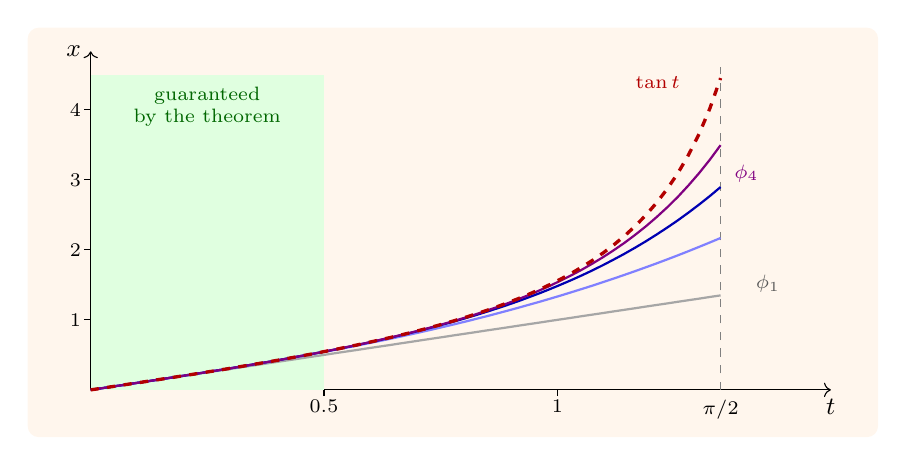
\begin{tikzpicture}[x=1cm,y=1cm]
\fill[orange!7,rounded corners=4pt] (-0.8,-0.6) rectangle (10.0,4.6);
\draw[->] (0,0) -- (9.4,0) node[below,font=\small] {$t$};
\draw[->] (0,0) -- (0,4.3) node[left,font=\small] {$x$};
\foreach \v/\x in {0.5/2.963, 1/5.926}
  \draw (\x,-0.08) -- (\x,0) node[below,font=\scriptsize] {$\v$};
\draw[dashed,gray] (8,0) -- (8,4.1);
\node[font=\scriptsize,below] at (8,0) {$\pi/2$};
\foreach \v/\y in {1/0.889, 2/1.778, 3/2.667, 4/3.556}
  \draw (-0.08,\y) -- (0,\y) node[left,font=\scriptsize] {$\v$};
\fill[green!12] (0,0) rectangle (2.963,4.0);
\node[font=\scriptsize,green!40!black,align=center] at (1.48,3.6) {guaranteed\\ by the theorem};
\draw[gray!70,thick] plot coordinates {(0.000,0.000) (0.136,0.020) (0.271,0.041) (0.407,0.061) (0.542,0.081) (0.678,0.102) (0.814,0.122) (0.949,0.142) (1.085,0.163) (1.220,0.183) (1.356,0.203) (1.492,0.224) (1.627,0.244) (1.763,0.264) (1.898,0.285) (2.034,0.305) (2.169,0.325) (2.305,0.346) (2.441,0.366) (2.576,0.386) (2.712,0.407) (2.847,0.427) (2.983,0.447) (3.119,0.468) (3.254,0.488) (3.390,0.508) (3.525,0.529) (3.661,0.549) (3.797,0.569) (3.932,0.590) (4.068,0.610) (4.203,0.631) (4.339,0.651) (4.475,0.671) (4.610,0.692) (4.746,0.712) (4.881,0.732) (5.017,0.753) (5.153,0.773) (5.288,0.793) (5.424,0.814) (5.559,0.834) (5.695,0.854) (5.831,0.875) (5.966,0.895) (6.102,0.915) (6.237,0.936) (6.373,0.956) (6.508,0.976) (6.644,0.997) (6.780,1.017) (6.915,1.037) (7.051,1.058) (7.186,1.078) (7.322,1.098) (7.458,1.119) (7.593,1.139) (7.729,1.159) (7.864,1.180) (8.000,1.200)};
\draw[blue!50,thick] plot coordinates {(0.000,0.000) (0.136,0.020) (0.271,0.041) (0.407,0.061) (0.542,0.082) (0.678,0.102) (0.814,0.123) (0.949,0.144) (1.085,0.165) (1.220,0.186) (1.356,0.207) (1.492,0.228) (1.627,0.250) (1.763,0.272) (1.898,0.294) (2.034,0.317) (2.169,0.340) (2.305,0.363) (2.441,0.387) (2.576,0.411) (2.712,0.435) (2.847,0.460) (2.983,0.485) (3.119,0.511) (3.254,0.537) (3.390,0.564) (3.525,0.591) (3.661,0.619) (3.797,0.647) (3.932,0.676) (4.068,0.706) (4.203,0.736) (4.339,0.767) (4.475,0.799) (4.610,0.831) (4.746,0.864) (4.881,0.898) (5.017,0.932) (5.153,0.968) (5.288,1.004) (5.424,1.041) (5.559,1.079) (5.695,1.117) (5.831,1.157) (5.966,1.197) (6.102,1.239) (6.237,1.281) (6.373,1.324) (6.508,1.369) (6.644,1.414) (6.780,1.461) (6.915,1.508) (7.051,1.557) (7.186,1.606) (7.322,1.657) (7.458,1.709) (7.593,1.762) (7.729,1.817) (7.864,1.872) (8.000,1.929)};
\draw[blue!70!black,thick] plot coordinates {(0.000,0.000) (0.136,0.020) (0.271,0.041) (0.407,0.061) (0.542,0.082) (0.678,0.102) (0.814,0.123) (0.949,0.144) (1.085,0.165) (1.220,0.186) (1.356,0.207) (1.492,0.229) (1.627,0.250) (1.763,0.272) (1.898,0.295) (2.034,0.318) (2.169,0.341) (2.305,0.364) (2.441,0.388) (2.576,0.413) (2.712,0.438) (2.847,0.463) (2.983,0.489) (3.119,0.516) (3.254,0.543) (3.390,0.571) (3.525,0.600) (3.661,0.630) (3.797,0.661) (3.932,0.692) (4.068,0.725) (4.203,0.759) (4.339,0.794) (4.475,0.830) (4.610,0.867) (4.746,0.906) (4.881,0.946) (5.017,0.988) (5.153,1.032) (5.288,1.077) (5.424,1.124) (5.559,1.174) (5.695,1.225) (5.831,1.279) (5.966,1.335) (6.102,1.393) (6.237,1.454) (6.373,1.518) (6.508,1.585) (6.644,1.656) (6.780,1.729) (6.915,1.806) (7.051,1.887) (7.186,1.972) (7.322,2.061) (7.458,2.154) (7.593,2.252) (7.729,2.355) (7.864,2.462) (8.000,2.576)};
\draw[violet,thick] plot coordinates {(0.000,0.000) (0.136,0.020) (0.271,0.041) (0.407,0.061) (0.542,0.082) (0.678,0.102) (0.814,0.123) (0.949,0.144) (1.085,0.165) (1.220,0.186) (1.356,0.207) (1.492,0.229) (1.627,0.250) (1.763,0.272) (1.898,0.295) (2.034,0.318) (2.169,0.341) (2.305,0.364) (2.441,0.388) (2.576,0.413) (2.712,0.438) (2.847,0.463) (2.983,0.490) (3.119,0.516) (3.254,0.544) (3.390,0.572) (3.525,0.601) (3.661,0.632) (3.797,0.663) (3.932,0.695) (4.068,0.728) (4.203,0.762) (4.339,0.798) (4.475,0.836) (4.610,0.874) (4.746,0.915) (4.881,0.957) (5.017,1.002) (5.153,1.049) (5.288,1.097) (5.424,1.149) (5.559,1.203) (5.695,1.261) (5.831,1.321) (5.966,1.386) (6.102,1.454) (6.237,1.526) (6.373,1.604) (6.508,1.686) (6.644,1.774) (6.780,1.868) (6.915,1.969) (7.051,2.077) (7.186,2.193) (7.322,2.318) (7.458,2.452) (7.593,2.598) (7.729,2.755) (7.864,2.924) (8.000,3.108)};
\draw[red!70!black,very thick,dashed] plot coordinates {(0.000,0.000) (0.136,0.020) (0.271,0.041) (0.407,0.061) (0.542,0.082) (0.678,0.102) (0.814,0.123) (0.949,0.144) (1.085,0.165) (1.220,0.186) (1.356,0.207) (1.492,0.229) (1.627,0.250) (1.763,0.272) (1.898,0.295) (2.034,0.318) (2.169,0.341) (2.305,0.364) (2.441,0.388) (2.576,0.413) (2.712,0.438) (2.847,0.463) (2.983,0.490) (3.119,0.516) (3.254,0.544) (3.390,0.572) (3.525,0.602) (3.661,0.632) (3.797,0.663) (3.932,0.695) (4.068,0.728) (4.203,0.763) (4.339,0.799) (4.475,0.837) (4.610,0.876) (4.746,0.917) (4.881,0.960) (5.017,1.005) (5.153,1.053) (5.288,1.103) (5.424,1.156) (5.559,1.212) (5.695,1.272) (5.831,1.337) (5.966,1.405) (6.102,1.479) (6.237,1.559) (6.373,1.645) (6.508,1.739) (6.644,1.842) (6.780,1.955) (6.915,2.080) (7.051,2.219) (7.186,2.375) (7.322,2.552) (7.458,2.753) (7.593,2.985) (7.729,3.255) (7.864,3.575) (8.000,3.960)};
\node[font=\scriptsize,red!70!black] at (7.2,3.9) {$\tan t$};
\node[font=\scriptsize,gray!70!black] at (8.6,1.35) {$\phi_1$};
\node[font=\scriptsize,violet,anchor=west] at (8.05,2.75) {$\phi_4$};
\end{tikzpicture}
\caption{Picard iterates $\phi_1, \dots, \phi_4$ for $x' = 1 + x^2$, $x(0) = 0$, against the solution $\tan t$. The iterates converge rapidly near $t = 0$ and ever more slowly towards $\pi/2$, where the
solution blows up. The shaded strip is the interval $[0, \frac12]$ that Theorem~\ref{thm:picard} guarantees.}
\label{fig:picard}
\end{figure}

\subhead{The contraction mapping view}
The proof is an instance of a general principle.

\begin{thm}[Banach]
\label{thm:banach}
Let $(X, d)$ be a complete metric space and $T\colon X \to X$ a contraction, $d(Tx, Ty) \leq q\,d(x, y)$ with $0 \leq q < 1$. Then $T$ has exactly one fixed point $x^*$, and for every $x_0 \in X$ the iterates
$x_{k+1} = Tx_k$ converge to it, with $d(x_k, x^*) \leq \frac{q^k}{1 - q}d(x_1, x_0)$.
\end{thm}

\begin{proof}
$d(x_{k+1}, x_k) \leq q^kd(x_1, x_0)$ by induction, so for $m > k$, $d(x_m, x_k) \leq \sum_{j=k}^{m-1}q^jd(x_1, x_0) \leq \frac{q^k}{1 - q}d(x_1, x_0)$: the sequence is Cauchy, and converges to some $x^*$ by
completeness. $T$ is continuous, so $Tx^* = \lim Tx_k = \lim x_{k+1} = x^*$. If $y^*$ is another fixed point, $d(x^*, y^*) = d(Tx^*, Ty^*) \leq q\,d(x^*, y^*)$, which forces $d(x^*, y^*) = 0$. Letting $m \to \infty$ in the
Cauchy estimate gives the error bound.
\end{proof}

To apply it, let $X$ be the set of continuous $\phi\colon J \to \bar B(x_0, b)$, which is complete under the uniform metric, and $T$ the integral operator. The cone argument shows $T(X) \subseteq X$.
With the ordinary sup norm, $\|T\phi - T\psi\|_\infty \leq L\alpha\|\phi - \psi\|_\infty$, a contraction only if $L\alpha < 1$. Bielecki (1956) removed this restriction with the weighted norm
$\|\phi\|_\ast = \sup_{t \in J}e^{-2L|t - t_0|}\|\phi(t)\|$, equivalent to the sup norm, in which $\|T\phi - T\psi\|_\ast \leq \frac12\|\phi - \psi\|_\ast$; this gives existence and uniqueness on all of $J$ in one
step (Problem~\ref{prob:bielecki}).

\subsection{Gronwall's inequality and continuous dependence}
\label{ssec:gronwall}

\begin{thm}[Gronwall]
\label{thm:gronwall}
Let $u$ be continuous and non-negative on $[t_0, t_1]$, and suppose that for constants $C \geq 0$ and $K \geq 0$,
\[
u(t) \leq C + K\int_{t_0}^tu(s)\,ds \qquad (t_0 \leq t \leq t_1) .
\]
Then $u(t) \leq Ce^{K(t - t_0)}$. More generally, if $u(t) \leq c(t) + \int_{t_0}^tk(s)u(s)\,ds$ with $k \geq 0$ continuous and $c$ continuous and non-decreasing, then
$u(t) \leq c(t)\exp\int_{t_0}^tk(s)\,ds$.
\end{thm}

\begin{proof}
We prove the general form. Let $v(t) = \int_{t_0}^tk(s)u(s)\,ds$, so $v' = ku \leq k(c + v)$. Fix $\tau \in [t_0, t_1]$; for $t \leq \tau$, $c(t) \leq c(\tau)$, so $v' - kv \leq kc(\tau)$. Multiplying by the integrating factor
$e^{-\int_{t_0}^tk}$ gives $\bigl(v e^{-\int_{t_0}^tk}\bigr)' \leq kc(\tau)e^{-\int_{t_0}^tk}$, and integrating from $t_0$ to $\tau$, with $v(t_0) = 0$,
\[
v(\tau)e^{-\int_{t_0}^\tau k} \leq c(\tau)\bigl(1 - e^{-\int_{t_0}^\tau k}\bigr), \qquad\text{that is}\qquad v(\tau) \leq c(\tau)\bigl(e^{\int_{t_0}^\tau k} - 1\bigr) .
\]
Then $u(\tau) \leq c(\tau) + v(\tau) \leq c(\tau)e^{\int_{t_0}^\tau k}$. The first statement is the case $c \equiv C$, $k \equiv K$.
\end{proof}

The inequality converts an integral inequality into an exponential bound, and it is the main tool for comparing solutions.

\begin{thm}[Continuous dependence]
\label{thm:contdep}
Let $f$ and $g$ be continuous on a region containing the graphs of $x(t)$ and $y(t)$, solutions of $x' = f(t, x)$, $x(t_0) = x_0$ and $y' = g(t, y)$, $y(t_0) = y_0$ on an interval $J \ni t_0$. If $f$ is
Lipschitz in $x$ with constant $L$ and $\|f(t, z) - g(t, z)\| \leq \varepsilon$ there, then for $t \in J$
\[
\|x(t) - y(t)\| \leq \|x_0 - y_0\|e^{L|t - t_0|} + \frac\varepsilon L\bigl(e^{L|t - t_0|} - 1\bigr) .
\]
\end{thm}

\begin{proof}
Take $t \geq t_0$. Subtracting the integral equations,
\[
x(t) - y(t) = x_0 - y_0 + \int_{t_0}^t\bigl[f(s, x) - f(s, y)\bigr]ds + \int_{t_0}^t\bigl[f(s, y) - g(s, y)\bigr]ds ,
\]
so $u = \|x - y\|$ satisfies $u(t) \leq \|x_0 - y_0\| + \varepsilon(t - t_0) + L\int_{t_0}^tu$. Put $w = u + \varepsilon/L$: then $w(t) \leq \|x_0 - y_0\| + \varepsilon/L + L\int_{t_0}^tw$, because $L\int_{t_0}^t\varepsilon/L = \varepsilon(t - t_0)$.
Gronwall gives $w(t) \leq (\|x_0 - y_0\| + \varepsilon/L)e^{L(t - t_0)}$, which rearranges to the claim.
\end{proof}

With $f = g$ the theorem says that solutions depend continuously, indeed Lipschitz-continuously, on their initial values, with a constant that may grow
like $e^{L|t - t_0|}$. With $x_0 = y_0$ it says that a small error $\varepsilon$ in the equation itself, a modelling error or a rounding error in a computation, produces an error at
time $t$ of at most $\varepsilon(e^{Lt} - 1)/L$. Together these make the initial value problem \textbf{well posed} in the sense of Hadamard: a solution exists, is unique, and
depends continuously on the data. The exponential factor is not an artefact: for $x' = Lx$ the bound is attained, and it is the root of the sensitivity of chaotic
systems studied at the end of the course.

\subsection{Peano's existence theorem}
\label{ssec:peano}

Continuity alone guarantees existence, though not uniqueness. The proof needs compactness in place of contraction.

\begin{thm}[Arzel\`a--Ascoli]
\label{thm:arzela}
A sequence of functions on a compact interval $J$ that is uniformly bounded and equicontinuous (for every $\varepsilon > 0$ there is $\delta > 0$ with $\|\phi_n(t) - \phi_n(s)\| < \varepsilon$ whenever
$|t - s| < \delta$, for all $n$) has a uniformly convergent subsequence.
\end{thm}

We take this standard result of analysis as known.

\begin{thm}[Peano]
\label{thm:peano}
If $f$ is continuous on $R$, the initial value problem has at least one solution on $J = [t_0 - \alpha, t_0 + \alpha]$.
\end{thm}

\begin{proof}
Take $t \geq t_0$. For each $n$, divide $[t_0, t_0 + \alpha]$ into $n$ steps of length $h = \alpha/n$ at $t_j = t_0 + jh$, and define the \textbf{Euler polygon} $\phi_n$ by $\phi_n(t_0) = x_0$ and
\[
\phi_n(t) = \phi_n(t_j) + (t - t_j)f\bigl(t_j, \phi_n(t_j)\bigr), \qquad t_j \leq t \leq t_{j+1} .
\]
By induction, as in the cone argument, each $\phi_n$ stays in $\bar B(x_0, b)$, and it is piecewise linear with slopes of norm at most $M$, so $\|\phi_n(t) - \phi_n(s)\| \leq M|t - s|$: the
sequence is uniformly bounded and equicontinuous. Writing $t_{[s]}$ for the grid point at or just below $s$,
\[
\phi_n(t) = x_0 + \int_{t_0}^tf\bigl(t_{[s]}, \phi_n(t_{[s]})\bigr)\,ds = x_0 + \int_{t_0}^tf\bigl(s, \phi_n(s)\bigr)\,ds + \int_{t_0}^t\delta_n(s)\,ds ,
\]
where $\delta_n(s) = f(t_{[s]}, \phi_n(t_{[s]})) - f(s, \phi_n(s))$. The two points at which $f$ is evaluated are within $h$ in $t$ and $Mh$ in $x$, and $f$ is uniformly continuous on the compact set $R$,
so $\|\delta_n\|_\infty \to 0$. By Theorem~\ref{thm:arzela} a subsequence $\phi_{n_k}$ converges uniformly to a continuous $\phi$; then $f(s, \phi_{n_k}(s)) \to f(s, \phi(s))$ uniformly, again by uniform
continuity, and passing to the limit gives $\phi(t) = x_0 + \int_{t_0}^tf(s, \phi(s))\,ds$. By Lemma~\ref{lem:integral}, $\phi$ is a solution.
\end{proof}

The proof constructs Euler's method and shows that a subsequence of its approximations converges. Without uniqueness, different subsequences may converge to
different solutions; with uniqueness, the whole sequence converges, and Euler's method is a convergent numerical scheme. Between Peano and Picard lie
weaker conditions for uniqueness. Osgood's (1898) criterion, $\|f(t, x) - f(t, y)\| \leq \omega(\|x - y\|)$ with $\int_0\frac{dr}{\omega(r)} = \infty$, covers $\omega(r) = r\log(1/r)$, which is not Lipschitz; the failing
example $3x^{2/3}$ has $\omega(r) = 3r^{2/3}$, for which the integral converges.

\subsection{Existence and uniqueness in software}
\label{ssec:software2}

\begin{software}[Picard iteration in SymPy]
\label{sw:picard}
The iterates of Example~\ref{ex:tanpicard}, computed by exact integration, compared with the Taylor series of $\tan t$:
{\small\begin{verbatim}
>>> import sympy as sp
>>> t, s = sp.symbols('t s')
>>> f = lambda t, x: 1 + x**2              # x' = 1 + x^2, x(0) = 0
>>> phi = [sp.Integer(0)]
>>> for k in range(4):                     # the Picard iteration
...     p = phi[-1].subs(t, s)
...     phi.append(sp.expand(sp.integrate(f(s, p), (s, 0, t))))
...
>>> phi[3]
t**7/63 + 2*t**5/15 + t**3/3 + t
>>> sp.series(sp.tan(t), t, 0, 9)
t + t**3/3 + 2*t**5/15 + 17*t**7/315 + O(t**9)
>>> [sp.degree(p, t) for p in phi[1:]]
[1, 3, 7, 15]
\end{verbatim}}
\textbf{Reading the output.} $\phi_3$ agrees with $\tan t = t + \frac{t^3}{3} + \frac{2t^5}{15} + \frac{17t^7}{315} + \cdots$ up to $t^5$; its $t^7$ coefficient $\frac{1}{63} = \frac{5}{315}$ is still wrong. The degrees $1, 3, 7, 15$ double
(plus one) at each step, because squaring a polynomial doubles its degree, so the iterates contain many wrong high-order terms that later steps correct.

\textbf{MATLAB/Octave:} \texttt{syms t s; p = sym(0); for k = 1:3, p = int(1 + subs(p, t, s)\^{}2, s, 0, t); end}.
\end{software}

\begin{software}[Convergence and the guaranteed interval]
\label{sw:picardconv}
The errors $\phi_k - \tan t$ at three times, and the best interval that Theorem~\ref{thm:picard} can promise over the choice of $b$:
{\small\begin{verbatim}
>>> import numpy as np
>>> xs = (0.25, 0.5, 1.0)
>>> for k in range(1, 5):
...     g = sp.lambdify(t, phi[k])
...     print(k, [round(float(g(x) - np.tan(x)), 5) for x in xs])
...
1 [-0.00534, -0.0463, -0.55741]
2 [-0.00013, -0.00464, -0.22407]
3 [-0.0, -0.00035, -0.07487]
4 [-0.0, -2e-05, -0.02045]
>>> b = np.linspace(0.01, 5, 2000); alpha = np.minimum(1.0, b / (1 + b**2))
>>> b[np.argmax(alpha)], alpha.max()
(1.0010105052526264, 0.49999974497761523)
\end{verbatim}}
\textbf{Reading the output.} At $t = 0.25$ and $t = 0.5$, inside the guaranteed interval, the error falls by an order of magnitude or more at each step; at $t = 1$, outside it,
convergence is slower but still visible ($-0.557$, $-0.224$, $-0.075$, $-0.020$). The iterates in fact converge on the whole of $(-\pi/2, \pi/2)$; the theorem is a sufficient condition,
not a description. The search over $b$ confirms that $\alpha = b/(1 + b^2)$ is maximised at $b = 1$, with $\alpha = \frac12$.

\textbf{MATLAB/Octave:} \texttt{b = linspace(0.01, 5, 2000); [amax, i] = max(min(1, b./(1 + b.\^{}2)))}.
\end{software}

\begin{software}[Continuous dependence and its failure]
\label{sw:dependence}
Two solutions of $x' = 2\sin x$ from initial values $0.001$ apart, against the bound of Theorem~\ref{thm:contdep}; then the equation $y' = 3y^{2/3}$ of Example~\ref{ex:nonunique} from $0$ and from $10^{-12}$:
{\small\begin{verbatim}
>>> from scipy.integrate import solve_ivp
>>> L, T = 2.0, 1.0                        # 2 sin x has Lipschitz L = 2
>>> rhs = lambda t, x: 2 * np.sin(x)
>>> x1 = solve_ivp(rhs, (0, T), [1.0], rtol=1e-11, atol=1e-12)
>>> x2 = solve_ivp(rhs, (0, T), [1.001], rtol=1e-11, atol=1e-12)
>>> gap = abs(x2.y[0, -1] - x1.y[0, -1]); gap, 0.001 * np.exp(L * T)
(0.0005542867025911669, 0.007389056098930651)
>>> nu = lambda t, y: 3 * np.cbrt(y)**2    # y' = 3 y^(2/3): uniqueness fails
>>> [solve_ivp(nu, (0, 1), [y0], rtol=1e-10, atol=1e-14).y[0, -1]
...  for y0 in (0.0, 1e-12)]
[0.0, 1.0003001102501183]
\end{verbatim}}
\textbf{Reading the output.} After one unit of time the two solutions are $0.00055$ apart, well within the Gronwall bound $0.001e^2 = 0.0074$; the bound allows for the worst case, in
which every direction is expanding at the maximal rate $L$, while near $x = 1$ the solutions are being drawn towards the stable equilibrium $\pi$. For the non-Lipschitz
equation, continuous dependence fails completely: starting at $0$ the solver returns $0$, but starting at $10^{-12}$ it follows $y \approx t^3$ to $y(1) = 1.0003$. An initial difference of
$10^{-12}$ has become a difference of $1$, because the two starting points lie on different members of the infinite family of solutions through the origin.

\textbf{MATLAB/Octave:} \texttt{[t, x] = ode45(@(t, x) 2*sin(x), [0 1], 1.001)}.
\end{software}

\subsection{Practice Problems}

\begin{problem}
Compute the Picard iterates for $x' = x$, $x(0) = 1$, and show that $\phi_k(t) = \sum_{j=0}^kt^j/j!$. What does Theorem~\ref{thm:picard} give as the interval of existence for $R$ with $a$ and $b$
arbitrary, and how does this compare with the truth?
\end{problem}

\begin{solution}
By induction, if $\phi_k = \sum_{j \leq k}t^j/j!$ then $\phi_{k+1} = 1 + \int_0^t\phi_k = 1 + \sum_{j \leq k}t^{j+1}/(j + 1)!$, the next partial sum. On $R$, $M = 1 + b$ (the maximum of $|x|$ for $|x - 1| \leq b$), so
$\alpha = \min(a, b/(1 + b))$, which is less than $1$ for every $b$. The theorem guarantees existence only on $|t| < 1$, although the solution $e^t$ exists for all $t$; global existence for linear
equations is proved in the next section.
\end{solution}

\begin{problem}
For $x' = t^2 + x^2$, $x(0) = 0$, on $R = \{|t| \leq 1, |x| \leq 1\}$, find $M$, $L$ and the interval of existence given by Theorem~\ref{thm:picard}. How many Picard iterates guarantee an error below
$10^{-6}$ on that interval?
\end{problem}

\begin{solution}
$M = \max(t^2 + x^2) = 2$, and $L = \max|\partial f/\partial x| = \max|2x| = 2$. Then $\alpha = \min(1, 1/2) = \frac12$. On $|t| \leq \frac12$, $L|t| \leq 1$, and the error bound is $\frac ML\frac{1}{(k + 1)!}e = \frac{e}{(k + 1)!}$. Since
$9! = 362\,880$ gives $7.5 \times 10^{-6}$ and $10! = 3\,628\,800$ gives $7.5 \times 10^{-7}$, $k + 1 = 10$, that is $k = 9$ iterates, suffice.
\end{solution}

\begin{problem}
Show that $x' = \sqrt{|x|}$, $x(0) = 0$, has infinitely many solutions, and that $x(0) = 1$ has a unique solution near $t = 0$. Reconcile the two with Theorem~\ref{thm:picard}.
\end{problem}

\begin{solution}
$x \equiv 0$ is a solution, and so is $x(t) = 0$ for $t \leq c$, $(t - c)^2/4$ for $t > c$, for every $c \geq 0$: on $t > c$, $x' = (t - c)/2 = \sqrt{x}$. Near $x = 1$, $\sqrt{|x|}$ is continuously differentiable,
so it is Lipschitz on a rectangle around $(0, 1)$ (Lemma~\ref{lem:c1lip}) and the theorem applies. The failure at $x = 0$ comes from $\frac{d}{dx}\sqrt x = \frac{1}{2\sqrt x}$ being unbounded there.
\end{solution}

\begin{problem}
Let $A(t)$ be a continuous $n \times n$ matrix function on $[t_0, t_1]$ and $x$ a solution of $x' = A(t)x$. Use Gronwall's inequality to show that
$\|x(t)\| \leq \|x(t_0)\|\exp\int_{t_0}^t\|A(s)\|\,ds$.
\end{problem}

\begin{solution}
$x(t) = x(t_0) + \int_{t_0}^tA(s)x(s)\,ds$, so $u = \|x\|$ satisfies $u(t) \leq \|x(t_0)\| + \int_{t_0}^t\|A(s)\|u(s)\,ds$. The general form of Theorem~\ref{thm:gronwall}, with $c \equiv \|x(t_0)\|$ and $k = \|A\|$, gives the bound. In
particular a solution of a linear system cannot blow up on a bounded interval, which is the key to global existence in the next section.
\end{solution}

\begin{problem}
The equation $x' = \sin x$ is solved twice from initial values $1$ and $1.01$. Bound the difference of the solutions on $[0, 2]$. A computer solves the equation with an error
of at most $10^{-8}$ in the right-hand side at every step; bound the resulting error at $t = 2$.
\end{problem}

\begin{solution}
$L = 1$. By Theorem~\ref{thm:contdep} with $\varepsilon = 0$, $|x(t) - y(t)| \leq 0.01e^t \leq 0.01e^2 = 0.074$ on $[0, 2]$. With equal initial values and $\varepsilon = 10^{-8}$, the error at $t = 2$ is at most
$10^{-8}(e^2 - 1) = 6.4 \times 10^{-8}$.
\end{solution}

\begin{problem}
For $y' = 3y^{2/3}$, $y(0) = 0$, compute the Picard iterates starting from $\phi_0 = 0$ and from $\phi_0 = t^3$. Explain why Banach's theorem does not apply.
\end{problem}

\begin{solution}
From $\phi_0 = 0$, every iterate is $0$. From $\phi_0 = t^3$, $\phi_1 = \int_0^t3(s^3)^{2/3}\,ds = \int_0^t3s^2\,ds = t^3$, so $t^3$ is also a fixed point. A contraction has only one fixed point, so the integral
operator is not a contraction in any metric of the kind used; the reason is the failure of the Lipschitz condition at $y = 0$ (Example~\ref{ex:lipschitz}(c)).
\end{solution}

\begin{problem}
\label{prob:bielecki}
With $\|\phi\|_\ast = \sup_{t \in J}e^{-2L|t - t_0|}\|\phi(t)\|$, show that the integral operator $T$ of Section~\ref{ssec:integral} satisfies $\|T\phi - T\psi\|_\ast \leq \frac12\|\phi - \psi\|_\ast$ under the Lipschitz condition.
\end{problem}

\begin{solution}
For $t \geq t_0$,
\begin{align*}
\|T\phi(t) - T\psi(t)\| &\leq L\int_{t_0}^te^{2L(s - t_0)}e^{-2L(s - t_0)}\|\phi(s) - \psi(s)\|\,ds\\
&\leq L\|\phi - \psi\|_\ast\int_{t_0}^te^{2L(s - t_0)}\,ds \leq \frac12\|\phi - \psi\|_\ast e^{2L(t - t_0)} .
\end{align*}
Multiplying by $e^{-2L(t - t_0)}$ and taking the supremum gives the result; $t < t_0$ is the same. Since $\|\cdot\|_\ast$ lies between $e^{-2L\alpha}\|\cdot\|_\infty$ and $\|\cdot\|_\infty$, the space is still complete, and
Banach's theorem gives a unique fixed point on the whole interval $J$, with no restriction $L\alpha < 1$.
\end{solution}

\section*{References}
\addcontentsline{toc}{section}{References}

\subhead{Principal texts}
\begin{enumerate}
\item Coddington, E. A., and Levinson, N. (1955), \emph{Theory of Ordinary Differential Equations}, New York, McGraw-Hill.
\item Hartman, P. (2002), \emph{Ordinary Differential Equations} (2nd ed.), Philadelphia, SIAM.
\item Hirsch, M. W., Smale, S., and Devaney, R. L. (2013), \emph{Differential Equations, Dynamical Systems, and an Introduction to Chaos} (3rd ed.),
Amsterdam, Academic Press.
\item Teschl, G. (2012), \emph{Ordinary Differential Equations and Dynamical Systems}, Providence, American Mathematical Society.
\end{enumerate}

\subhead{Recommended texts}
\begin{enumerate}
\item Arnold, V. I. (1992), \emph{Ordinary Differential Equations}, Berlin, Springer.
\item Perko, L. (2001), \emph{Differential Equations and Dynamical Systems} (3rd ed.), New York, Springer.
\item Strogatz, S. H. (2015), \emph{Nonlinear Dynamics and Chaos} (2nd ed.), Boulder, Westview Press.
\end{enumerate}

\subhead{Software}
\begin{enumerate}
\item Harris, C. R., et al. (2020), Array programming with NumPy, \emph{Nature}, 585, 357--362.
\item Meurer, A., et al. (2017), SymPy: symbolic computing in Python, \emph{PeerJ Computer Science}, 3, e103.
\item Virtanen, P., et al. (2020), SciPy 1.0: fundamental algorithms for scientific computing in Python, \emph{Nature Methods}, 17, 261--272.
\end{enumerate}

\subhead{Further reading}
\begin{enumerate}
\item Banach, S. (1922), Sur les op\'erations dans les ensembles abstraits et leur application aux \'equations int\'egrales, \emph{Fundamenta
Mathematicae}, 3, 133--181.
\item Bielecki, A. (1956), Une remarque sur la m\'ethode de Banach--Cacciopoli--Tikhonov dans la th\'eorie des \'equations diff\'erentielles
ordinaires, \emph{Bulletin de l'Acad\'emie Polonaise des Sciences}, 4, 261--264.
\item Gronwall, T. H. (1919), Note on the derivatives with respect to a parameter of the solutions of a system of differential equations,
\emph{Annals of Mathematics}, 20, 292--296.
\item Kermack, W. O., and McKendrick, A. G. (1927), A contribution to the mathematical theory of epidemics, \emph{Proceedings of the Royal Society of
London, Series A}, 115, 700--721.
\item Lindel\"of, E. (1894), Sur l'application de la m\'ethode des approximations successives aux \'equations diff\'erentielles ordinaires du
premier ordre, \emph{Comptes Rendus de l'Acad\'emie des Sciences}, 118, 454--457.
\item Lotka, A. J. (1925), \emph{Elements of Physical Biology}, Baltimore, Williams and Wilkins.
\item Osgood, W. F. (1898), Beweis der Existenz einer L\"osung der Differentialgleichung $dy/dx = f(x, y)$ ohne Hinzunahme der Cauchy-Lipschitz'schen
Bedingung, \emph{Monatshefte f\"ur Mathematik und Physik}, 9, 331--345.
\item Peano, G. (1890), D\'emonstration de l'int\'egrabilit\'e des \'equations diff\'erentielles ordinaires, \emph{Mathematische Annalen}, 37,
182--228.
\item Picard, \'E. (1890), M\'emoire sur la th\'eorie des \'equations aux d\'eriv\'ees partielles et la m\'ethode des approximations successives,
\emph{Journal de Math\'ematiques Pures et Appliqu\'ees}, 6, 145--210.
\item Verhulst, P.-F. (1838), Notice sur la loi que la population suit dans son accroissement, \emph{Correspondance Math\'ematique et Physique}, 10,
113--121.
\item Volterra, V. (1926), Fluctuations in the abundance of a species considered mathematically, \emph{Nature}, 118, 558--560.
\end{enumerate}

\end{document}
